\documentclass[11pt]{article}
\ifdefined\pdfgentounicode
\pdfgentounicode=1
\input{glyphtounicode-cmex}
\fi
\usepackage[T1]{fontenc}
\usepackage{lmodern}
\usepackage[margin=1in]{geometry}
\usepackage{amsmath,amssymb,amsthm,mathtools,bm}
\usepackage{microtype,enumitem,booktabs}
\usepackage{flafter}
\usepackage{placeins}
\usepackage{tikz}
\usetikzlibrary{arrows.meta,positioning,decorations.pathreplacing}
\usepackage[hyphens]{url}
\usepackage[colorlinks=true,linkcolor=black,citecolor=black,urlcolor=black]{hyperref}
\hypersetup{pdftitle={Computing the Random 3-SAT Threshold},pdfauthor={OpenAI},bookmarksdepth=2}
\newcommand{\E}{\mathbb E}
\newcommand{\Prob}{\mathbb P}
\newcommand{\R}{\mathbb R}
\newcommand{\N}{\mathbb N}
\newcommand{\Poi}{\operatorname{Poi}}
\newcommand{\Var}{\operatorname{Var}}
\newcommand{\1}{\mathbf 1}
\newcommand{\dd}{\,\mathrm d}
\newcommand{\TV}{\operatorname{TV}}
\newcommand{\Lip}{\operatorname{Lip}}
\newcommand{\supp}{\operatorname{supp}}
\newtheorem{theorem}{Theorem}[section]
\newtheorem{lemma}[theorem]{Lemma}
\newtheorem{proposition}[theorem]{Proposition}
\newtheorem{corollary}[theorem]{Corollary}
\theoremstyle{definition}
\newtheorem{definition}[theorem]{Definition}
\theoremstyle{remark}
\newtheorem{remark}[theorem]{Remark}
\numberwithin{equation}{section}
\setlist{itemsep=2pt,topsep=5pt}
\setcounter{tocdepth}{1}
\title{Computing the Random 3-SAT Threshold}
\author{OpenAI}
\date{September 27, 2026}
\begin{document}
\maketitle
\begin{abstract}
The limiting satisfiability threshold of uniform random 3-SAT is a
computable real. We credit Gaia Carenini~\cite{Carenini2026Polynomial}
with priority for resolving the satisfiability conjecture, which
establishes the threshold's existence. We prove that one finite
deterministic machine can approximate it to any prescribed accuracy. A deletion estimate gives
explicit lower certificates, while a finite hierarchical approximation
of the soft pressure gives upper certificates at every larger rational
density. A fair search through these certificates halts without
requiring a computable rate of finite-size convergence.
\end{abstract}
\section{Introduction}\label{sec:introduction}

For $n\ge3$, a proper random 3-clause chooses three distinct variables
uniformly from $x_1,\ldots,x_n$ and gives each variable an independent
fair sign. Let $\Phi(n,m)$ be the conjunction of $m\ge0$ independent
clauses with this law. Thus its clauses are sampled with replacement
from the $8\binom n3$ possibilities; the formula with no clauses is
satisfiable. Write
\[
 p(n,m)=\Prob\{\Phi(n,m)\text{ is satisfiable}\}.
\]
The ratio $m/n$ is the clause density. We prove that the limiting density
separating satisfiable and unsatisfiable formulas can be approximated to
any prescribed accuracy by one finite algorithm.

Carenini~\cite[Corollary~1.2]{Carenini2026Polynomial} establishes the
existence of a limiting satisfiability threshold for every fixed
$k\ge3$. We credit Carenini with priority for the resolution of the
satisfiability conjecture. The contribution here is computability of
the 3-SAT threshold, beyond its existence.

\begin{theorem}\label{thm:main}
There is a real number $\alpha_3\in(0,\infty)$ such that, for every fixed
real $a\ge0$,
\[
 \lim_{n\to\infty}p(n,\lfloor an\rfloor)=
 \begin{cases}1,&a<\alpha_3,\\0,&a>\alpha_3.\end{cases}
\]
There is one finite deterministic Turing machine which, on input $1^r$
for any integer $r\ge1$, halts with a rational number $q_r$ satisfying
$|q_r-\alpha_3|\le2^{-r}$. Its only input is the unary precision $1^r$;
it uses no oracle, advice, or noncomputable real constant.
\end{theorem}

The strict-side limits determine $\alpha_3$ uniquely, since two different
constants would give opposite limits at a density between them. The
theorem leaves the behavior at $a=\alpha_3$ open. Its algorithm computes
the limiting density; it does not search for satisfying assignments to
an input formula. We obtain no efficiency bound, and the computability
argument concerns clause size three.

Random 3-SAT has long served as a test case for the typical behavior of
satisfiability problems. Experiments of Mitchell, Selman, and
Levesque~\cite{MSL1992} placed difficult instances for the Davis--Putnam
procedure near the density where half the formulas were satisfiable.
Algorithmic and counting arguments then constrained the transition's
location. Kaporis, Kirousis, and Lalas~\cite{KaporisKirousisLalas2006}
obtained the lower bound $3.52$, independently reported by Hajiaghayi
and Sorkin~\cite{HajiaghayiSorkin2003}; D\'iaz, Kirousis, Mitsche, and
P\'erez-Gim\'enez~\cite{DiazKirousisMitschePerezGimenez2009} obtained the
upper bound $4.4898$. These bounds bracket any limiting threshold.
From statistical physics, M\'ezard, Parisi, and Zecchina developed the
cavity and survey-propagation description~\cite{MPZ2002}. The
calculations of M\'ezard and Zecchina~\cite{MZ2002}, refined by Mertens,
M\'ezard, and Zecchina~\cite{MMZ2006}, predict a threshold near $4.267$.
Theorem~\ref{thm:main}
establishes existence and computability without evaluating the constant
or identifying it with that prediction.

Two further distinctions explain the mathematical task. A transition
window can become narrow while its center still varies with the system
size. Friedgut's theorem, with Bourgain's appendix~\cite{Friedgut1999},
establishes a sharp transition for every fixed $k\ge3$ about a
size-dependent location. In earlier work,
Carenini~\cite[Corollaries~7.10--7.11]{Carenini} obtained an
$O(n/\log n)$ central clause window for each fixed $k\ge3$, including
the model with independently sampled proper clauses. Her polynomial
improvement to $O_{k,\eta}(n^{1/2+1/k})$ between probability levels
$\eta$ and $1-\eta$, for each fixed $0<\eta<1/2$, in
\cite[Theorem~1.1]{Carenini2026Polynomial} yields limiting thresholds
for every fixed $k\ge3$.
Bayati, Gamarnik, and Tetali~\cite{BGT2013} developed sparse
interpolation and proved limits for normalized optimization values and
finite-temperature normalized log partition functions. Their near-satisfiability
conclusion permits $o(n)$ violated clauses; exact satisfiability requires
none. Ding, Sly, and Sun~\cite{DSS2022} proved the
limiting-threshold conjecture, including the predicted value, for all
sufficiently large fixed clause sizes. The probability argument below
also proves existence at clause size three as part of the development
of the computability result.

Even when a finite-size limit exists, it need not be a computable real.
Specker~\cite[Satz~IV]{Specker1949} constructed a bounded nondecreasing
computable sequence of rationals with a noncomputable limit. Our proof
supplies two families of finite certificates. The first certifies
rational lower bounds on $\alpha_3$ that approach it arbitrarily closely.
The second certifies rational upper bounds, with a certificate at every
rational density strictly above $\alpha_3$. A fair search through both
families produces certified intervals of arbitrarily small length. Its
stopping rule uses the certified interval itself and requires no
convergence modulus for the finite-size quantities.

\section{Two certificate searches give a computable real}\label{sec:certificates}

The following elementary lemma isolates the effective part of the proof.
Its test value $G(a,\beta;Q)$ is an arbitrary computable real satisfying
the two stated sign conditions. The random-formula construction will
supply those conditions; the search itself uses only finite strings and
certified rational approximations.

\begin{lemma}[Finite-certificate search]\label{cert:search}
Let $\alpha\in[0,20]$. Suppose that $(\ell_k)_{k\ge1}$ is a computable
sequence of rational numbers satisfying $\ell_k\le\alpha$ for every $k$
and $\ell_k\to\alpha$. Suppose also that finite descriptions $Q$ form
an effectively enumerable class, and that for every positive rational
$a$, positive integer $\beta$, and valid description $Q$, the real number
$G(a,\beta;Q)$ is uniformly computable. Assume that
\begin{enumerate}
\item $G(a,\beta;Q)<0$ implies $\alpha\le a$;
\item for every rational $a>\alpha$, some positive integer $\beta$ and
      valid description $Q$ satisfy $G(a,\beta;Q)<0$.
\end{enumerate}
Then one finite deterministic Turing machine, with only the unary input
$1^r$ for $r\ge1$, returns a rational number within $2^{-r}$ of $\alpha$.
It can encode the output as a binary integer numerator and a positive
integer denominator, with separators.
\end{lemma}

\begin{proof}
Uniform computability gives, from $(a,\beta,Q)$ and an accuracy index,
a rational closed interval containing $G(a,\beta;Q)$ whose width tends
to zero as the index increases. If $G(a,\beta;Q)<0$, one such interval
has a strictly negative upper endpoint. This semidecides strict
negativity without testing equality to zero.

Start with $[l,u]=[0,20]$. Fix an effective enumerator of the triples
$(a,\beta,Q)$ in the statement. At stage $s$, run it for $s$ computation
steps from its start. For every triple emitted during those steps,
compute its value intervals at all accuracy indices at most $s$, and
compute $\ell_1,\ldots,\ell_s$. This is a finite list of terminating
computations. Replace $l$ by the maximum of its old value and the lower
certificates just computed. Whenever a value interval has a strictly
negative upper endpoint, replace $u$ by $\min\{u,a\}$. After each update,
if $u-l\le2^{1-r}$, output $(u+l)/2$ and halt.

Every interval maintained by the procedure contains $\alpha$. Its lower
endpoint does so by the hypothesis on $\ell_k$, and its upper endpoint
does so by assumption (1). To prove termination, fix $\varepsilon>0$.
Some $\ell_k>\alpha-\varepsilon$ is eventually computed. Choose a positive
rational $a$ with $\alpha<a<\alpha+\varepsilon$. By assumption (2), a
particular triple at this density has a negative value. The enumerator
emits this triple after finitely many steps, and some finite accuracy
index certifies its negativity. Both are processed at a finite stage.
Thereafter $l>\alpha-\varepsilon$ and $u<\alpha+\varepsilon$.
The interval length tends to zero, so the stopping test succeeds for
every $r$. Its midpoint has error at most $2^{-r}$.

All operations in this schedule act on finite integer and rational
encodings. The algorithms supplied by the hypotheses are fixed parts of
one program. The density and witness chosen in the termination argument
are not advice given to that program.
\end{proof}

\section{Where the certificates come from}\label{sec:proof-map}

The probability argument first constructs a threshold $\alpha$ for the
same proper clause law as in Theorem~\ref{thm:main}. It therefore equals
the $k=3$ constant of \emph{A Limiting Satisfiability Threshold for Every
Fixed Clause Size}~\cite[Theorem~1.1]{FixedClauseThreshold}: different
constants would force opposite limits at a density between them. The
comparison identifies the constants. We give the probability argument
locally because the computation needs two additional conclusions:
explicit lower certificates and a positive density of unavoidable
violations above the threshold.

\paragraph{Lower certificates and the sign of pressure.}
For this part of the proof, clauses arrive in a rate-one Poisson process
and their three variable indices are sampled independently, so indices
may repeat within a clause. Let $T_n$ be the first unsatisfiable arrival
time and put $f_n=\E\min\{T_n,20n\}$. Section~\ref{cp:section} proves
\[
 \frac{f_n}{n}\longrightarrow\alpha,
 \qquad \frac{f_n}{n}-2^{67}n^{-1/6}\le\alpha.
\]
Each $f_n$ admits certified rational approximations by finite clause
enumeration and integration. These facts give a computable sequence of
rational lower certificates converging to $\alpha$. Thinning and a
comparison with fixed density slack transfer the threshold from the
auxiliary law to proper clauses.

The estimate behind these conclusions bounds the extra survival time
when one variable may be deleted for free. Its $6/5$ moment is bounded
uniformly even when other deletions are already allowed. The replacement
step follows the residual-set conditioning principle of Friedgut's
half-cube lemma~\cite[Lemma~5.7]{Friedgut1999} and Carenini's sequential
clause replacement~\cite[Theorem~4.3 and Lemma~6.1]{Carenini}. Here
independent variable positions give exact powers for two-literal and
three-literal killing probabilities. A weighted interpolation between
unequal blocks, followed by a weight-balancing argument, turns the moment
bound into a summable error in the normalized mean. Keeping the existing
deletion allowance has a second use: above $\alpha$, every assignment
violates a positive multiple of $n$ clauses with probability tending to
one.

For the auxiliary Poisson formula at time $an$, let $H_n(\sigma)$ count
the clauses violated by an assignment $\sigma$. For a finite penalty
$\beta>0$, define
\[
 Z_n(a,\beta)=\sum_{\sigma\in\{0,1\}^n}e^{-\beta H_n(\sigma)},
 \qquad
 P(a,\beta)=\lim_{n\to\infty}\frac1n\E\log Z_n(a,\beta).
\]
Section~\ref{ctr:section} proves that this pressure limit exists. Below
$\alpha$ it is nonnegative for every $\beta>0$. Above $\alpha$, the
linear violation bound makes it strictly negative for some positive
integer $\beta$.

\paragraph{Finite upper certificates.}
The remaining task is to detect negative pressure using finite data.
Section~\ref{ctr:section} defines an effectively enumerable family of
rational trial descriptions. A description consists of finitely many
rational averaging parameters and a finite table of rational pairs in
$[0,1]^2$. The two coordinates give messages for the two literal signs;
they need not sum to one. Independent uniform coordinates select table
entries through finitely many conditional sampling levels. Different
sites may share initial random data, called the root data, but their
subsequent coordinates are independent. The value $G(a,\beta;Q)$ of a
trial is uniformly computable, and we prove
\[
 P(a,\beta)\le G(a,\beta;Q),\qquad
 P(a,\beta)=\inf_Q G(a,\beta;Q).
\]
A certified negative value is therefore an upper certificate for
$\alpha$, and the infimum identity supplies one at every rational
density above $\alpha$.

The inequality and the infimum identity require different arguments.
For the inequality, the three-literal interpolation leaves the
nonnegative remainder $(x-y)^2(x+2y)$ for $x,y\ge0$. For the reverse
approximation, finite formulas produce nearly optimal trials, but their
later sampling levels can still share random variables between sites.
Removing those variables is the main structural task. Conditional
changes of sampling law and Gaussian tests describe the continuation
law of a fresh site for almost every fixed history of the shared
coordinates. This qualification lets the description survive later
changes of law.

Section~\ref{cs:section} first proves that changing all averaging
parameters has a cost independent of the number of levels. This lets
the tolerances be chosen before the number of structural reductions is
known. Section~\ref{ct:section} then obtains the conditional descriptions
needed by those reductions. Each reduction either reaches the root or
decreases the first remaining parameter by a fixed factor. After
finitely many steps, Section~\ref{cc:section} samples the retained
conditional laws independently at each site, controls the change of the
trial value, and approximates the resulting kernels by finite rational
tables.

Finite hierarchical trials developed in the diluted interpolation and
cavity tradition of Franz and Leone~\cite{FranzLeone2003}, Panchenko
and Talagrand~\cite{PanchenkoTalagrand2004}, and Aizenman, Sims, and
Starr~\cite{AizenmanSimsStarr2003}. The upper-bound and reservoir
calculations below use their interpolation and cavity mechanisms in the
present three-literal model. Panchenko's ultrametricity theorem and the
hierarchical representation of Austin and
Panchenko~\cite{Panchenko2013UM,AustinPanchenko2014} supply the geometry
and representation of the limiting random arrays. Panchenko's pure-state
analysis~\cite{Panchenko2015HE} motivates the identities that also test
the retained site data. The conditional-law records then control
replacement of shared nonroot coordinates by independent site sampling.
This approximation, followed by rational discretization, gives the finite
trial completeness needed for the certificate search.

The proof may select subsequences and conditional laws non-effectively.
Those selections establish that a finite witness exists. The algorithm
searches finite descriptions; it does not receive a selected law or a
convergence modulus. Section~\ref{sec:assembly} closes the argument by
checking the two hypotheses of Lemma~\ref{cert:search}.

\clearpage
\tableofcontents
\section{Probability estimates for the two certificate searches}
\label{cp:section}

The certificate search needs two facts about random formulas. First, it
needs computable lower bounds that approach the limiting density. Second,
it needs a nonnegative lower limit below the threshold and a negative
upper limit above it for normalized expected log partition functions,
with a suitable finite penalty in the latter case. These become pressure
signs when the pressure limit is established. The common
estimate controls the extra time for which a formula stays satisfiable
when one variable may be deleted, even if other deletions are already
allowed.

It is useful to begin with an auxiliary clause law. For every integer
$n\ge1$, clauses arrive in a Poisson process of rate one. Each of their three variable
indices is sampled independently and uniformly from $[n]$, and each sign
is sampled independently and fairly. All indices, signs, and the clock
are independent. Repetitions \emph{within} a clause are permitted; time
$an$ therefore gives a Poisson number of these clauses with mean $an$.
We call this the \emph{relaxed Poisson model}. Later in the section we
transfer its strict-side limits to the proper-clause model of the
introduction.

Fix throughout this section
\begin{equation}\label{cp:constants}
 B=20,\qquad p=\frac65,\qquad b=\frac1p=\frac56.
\end{equation}
For an integer $r$ with $0\le r\le n$, a formula is called $r$-deletion satisfiable if some set
of at most $r$ variables can be deleted so that the remaining formula is
satisfiable; deleting a variable discards every clause that touches it.
Let $T_r$ be the first time $r$-deletion satisfiability fails, with
$T_r=+\infty$ if it never fails, and put
\[
 F_r=T_r\wedge Bn.
\]
The formula at time $t$ includes all arrivals up to and including $t$.
Accordingly it survives at time $t$ exactly when $T_r>t$. For a fixed
variable $v$, a superscript $+v$ means that $v$ is deleted for free and up
to $r$ \emph{other} variables may be deleted. In particular,
$F_r^{+v}=T_r^{+v}\wedge Bn\ge F_r$, with the same cap $Bn$.
Allowing more deletions than there are other variables
has its literal meaning; it simply permits deleting all of them.
We suppress the dependence on $n$ in these times.  For this fixed size,
the overview's $T_n$ is $T_0$ here; both denote the uncapped first-unsatisfiable
time, whereas $F_0=T_0\wedge Bn$ is capped.  Write
\[
 f_n=\E F_0,\qquad P_n(t)=\Prob(T_0>t).
\]
Thus $f_n$ is the mean first-unsatisfiable time capped at $20n$.

\subsection{A uniform moment bound for one free deletion}

\begin{lemma}[Free-deletion moment]\label{cp:deletion-moment}
For all integers $n\ge1$ and $0\le r\le n$, and every $v\in[n]$,
\begin{equation}\label{cp:one-delay}
 \E\bigl[(F_r^{+v}-F_r)^p\bigr]\le C,\qquad C=2^{60}.
\end{equation}
Consequently, uniformly in $r$,
\begin{equation}\label{cp:concentration}
 \E\lvert F_r-\E F_r\rvert^p\le C_1n,
 \qquad C_1=2^{62}.
\end{equation}
\end{lemma}

The proof compares two ways to eliminate a set of surviving assignments.
Clauses containing the free variable once become two-literal tests after
that variable is fixed. A batch of relaxed three-literal tests can replace
each such test at controlled loss. This is the residual-set conditioning
principle used in Friedgut's half-cube lemma
\cite[Lemma~5.7]{Friedgut1999} and in Carenini's sequential clause
replacement \cite[Theorem~4.3 and Lemma~6.1]{Carenini}. The calculation
below is for independently sampled positions: their exact powers give
the estimate needed under an existing deletion allowance.

\begin{proof}
For $n=1$, Equation~\eqref{cp:one-delay} follows directly from
$0\le F_r^{+v}-F_r\le20$. Suppose henceforth that $n\ge2$.

\emph{Incident clauses.}
Split the Poisson process into the clauses avoiding $v$, called the
\emph{base}, and the clauses involving $v$. The base has rate
\[
 \lambda_n=\left(\frac{n-1}{n}\right)^3\ge\frac18,
\]
and its clauses have the relaxed distribution on the other $n-1$ variables.
It is independent of the incident streams.

At a deterministic time $t$, condition on the entire base up to $t$.
Let $U_t$ be its finite set of surviving pairs $(D,\sigma)$, where
$D\subseteq[n]\setminus\{v\}$ has size at most $r$ and $\sigma$ is an
assignment on $[n]\setminus(D\cup\{v\})$. When a literal is tested on such a
pair, a literal on $D$ is declared true. This convention exactly implements
clause deletion. The event $U_t\ne\varnothing$ is $\{T_r^{+v}>t\}$.
For a nonempty deterministic candidate set $U$, let $q(U)$ be the probability
that $\Poi(K)$ independent relaxed two-literal clauses on the other
variables eliminate every candidate, where $K=3B=60$.

For $0\le t<Bn$ and $U_t\ne\varnothing$, we claim
\begin{equation}\label{cp:incident-killing}
 \Prob(T_r\le t\mid\text{base up to }t)
 \le \bigl(q(U_t)+60/n\bigr)^2.
\end{equation}
To check this, fix a value for $v$. Only incident clauses in which every
occurrence of $v$ has the sign falsified by that value can obstruct an
extension of a candidate in $U_t$. Among these clauses, those containing
$v$ once project to independent relaxed two-literal clauses. Their number
is Poisson with mean at most $3t/n\le60$. The expected number containing
$v$ at least twice is at most $3t/n^2\le60/n$, by a union bound over the
three pairs of positions. The obstruction probability for this value is
therefore at most $q(U_t)+60/n$. The obstructing groups for the two values
of $v$ are disjoint Poisson thinnings, hence independent of one another
and of the base. If either group leaves a candidate, restoring $v$ with
that value gives an $r$-deletion satisfying assignment. Both groups must
therefore obstruct, which proves Equation~\eqref{cp:incident-killing}.

\emph{Replacing shorter tests.}
In any list of
independent tests, replacing one relaxed two-literal clause by $d\ge1$
independent relaxed three-literal clauses reduces the probability of
eliminating all candidates by at most $d^{-2}$. Indeed, condition on all
other tests, leaving a candidate set $U'$. There is nothing to prove if it
is empty. Otherwise let $x$ be the proportion of signed literals false on
every member of $U'$. Each variable contributes at most one such sign, so
$0\le x\le1/2$, including under the deleted-literal convention. The
two-literal clause alone eliminates $U'$ with probability $x^2$. The $d$
three-literal clauses do so with probability at least
$1-(1-x^3)^d\ge1-e^{-dx^3}$. If $dx^3>1$, this lower bound exceeds
$1/4\ge x^2$. If $dx^3\le1$, it is at least $dx^3/2$, and
\[
 x^2-\frac d2x^3\le\frac{16}{27d^2}<\frac1{d^2}.
\]
This proves the comparison. Applying it successively is valid because,
at each replacement, one can condition on all the other independent tests.

\emph{How long a residual set can survive.}
The replacement estimate converts a large value of $q(U_t)$ into a
chance that the future base eliminates $U_t$. Partition the possible
values $q(U_t)\ge1/n$ into disjoint dyadic bins
$q_0\le q(U_t)\le2q_0$, with $q_0=2^{-j}$ and $j\ge1$, using any
fixed endpoint convention. Every bin that is used has $q_0\ge1/(2n)$.
For its index $j$, set
\begin{equation}\label{cp:bin-parameters}
 L_j=j+122,\qquad
 d_j=\left\lceil\sqrt{4L_j/q_0}\right\rceil,\qquad
 \ell_j=32L_jd_j.
\end{equation}
Since $\E2^{\Poi(60)}=e^{60}<2^{120}$,
$\Prob(\Poi(60)>L_j)\le q_0/4$. If $U$ belongs to the bin, then
$L_j$ two-literal tests eliminate it with probability at least
$q(U)-q_0/4$. Replacing each test by $d_j$ three-literal tests loses at
most $L_j/d_j^2\le q_0/4$. Thus $L_jd_j$ three-literal tests eliminate
$U$ with probability at least $q_0/2$.

In a future interval of length $\ell_j$, the base has a Poisson number of
arrivals with mean at least $4L_jd_j$. If $M=L_jd_j\ge1$ and $X$ is
Poisson with mean $\mu\ge4M$, Chebyshev's inequality gives
\[
 \Prob(X<M)\le\frac{\mu}{(\mu-M)^2}
 \le\frac4{9M}<\frac12.
\]
Consequently this interval eliminates the fixed $U$ with probability at
least $q_0/4$. Write
\[
 S_{r,v}(t)=\Prob(T_r^{+v}>t),\qquad
 E_j(t)=\{U_t\ne\varnothing,\ q(U_t)\text{ belongs to bin }j\}.
\]
The independent future base then gives
\begin{equation}\label{cp:bin-time}
 \begin{split}
 S_{r,v}(t)-S_{r,v}(t+\ell_j)&\ge(q_0/4)\Prob(E_j(t)),\\
 \int_0^{Bn}\Prob(E_j(t))\,\dd t&\le4\ell_j/q_0.
 \end{split}
\end{equation}
For the second inequality, integrate the first: the integral of
$S_{r,v}(t)-S_{r,v}(t+\ell_j)$ over $[0,Bn]$ is at most $\ell_j$.
This argument does not require $T_r^{+v}$ to be finite. Conditional on the
base at time $t$ in $E_j(t)$, survival to $t+u$ is also bounded by
\begin{equation}\label{cp:bin-survival}
 (1-q_0/4)^{\lfloor u/\ell_j\rfloor}.
\end{equation}
For each complete future interval, failure to eliminate even the original
$U_t$ is necessary for survival; these interval events are independent.

\emph{Integrating the delay.}
For any $0\le F_r\le F_r^{+v}\le Bn$, direct integration gives the
pathwise identity
\begin{equation}\label{cp:delay-integral}
 (F_r^{+v}-F_r)^p
 =p(p-1)\int_{\substack{t,u\ge0\\t+u<Bn}}
 u^{p-2}\1_{\{T_r\le t,\ T_r^{+v}>t+u\}}\,\dd t\,\dd u.
\end{equation}
The boundaries have Lebesgue measure zero, so a hitting time equal to the
cap causes no difficulty. Conditional on the base up to $t$, incident
arrivals up to $t$ and future base arrivals are independent. The incident
killing estimate~\eqref{cp:incident-killing} and the future survival
estimate~\eqref{cp:bin-survival} therefore multiply.

Here is why the resulting sum over bins converges. On a bin of scale
$q_0$, incident killing has probability at most a constant times $q_0^2$.
The expected total time spent in that bin before $Bn$ is at most
$4\ell_j/q_0$, by
Equation~\eqref{cp:bin-time}. Integrating the geometric future-survival
bound against $u^{p-2}$ contributes at most a constant times
$(\ell_j/q_0)^{p-1}$. Thus the bin contribution is bounded by a constant times
$\ell_j^p q_0^{2-p}$. Since $\ell_j$ grows like a polynomial in $j$ times
$q_0^{-1/2}$, the power of $q_0$ is $2-3p/2=1/5>0$.

We now retain explicit constants for the later one-sided certificate.
On bin $j$,
\[
 (q(U_t)+60/n)^2\le(122q_0)^2<2^{14}q_0^2,
 \qquad
 \ell_j\le2^{20}(j+1)^{3/2}2^{j/2}.
\]
For the latter, $d_j\le3\sqrt{L_j/q_0}$ and
$L_j\le64(j+1)$ suffice. Moreover,
\[
 \begin{split}
 &\int_0^\infty u^{p-2}
     (1-q_0/4)^{\lfloor u/\ell_j\rfloor}\,\dd u\\
 &\qquad\le
 e\,\Gamma(1/5)(4\ell_j/q_0)^{1/5}
 <2^7(\ell_j/q_0)^{p-1}.
 \end{split}
\]
Indeed, the geometric term is at most
$e\exp(-q_0u/(4\ell_j))$, and splitting the defining Gamma integral
at $1$ gives $\Gamma(1/5)<6$. Using
Equation~\eqref{cp:bin-time} and $p(p-1)<1$, the contribution of bin $j$
to the expectation in Equation~\eqref{cp:delay-integral} is at most
\[
 2^{47}(j+1)^2\,2^{-j/5}.
\]
Grouping $j=5k+1,\ldots,5k+5$ gives
\[
 \sum_{j\ge1}(j+1)^2\,2^{-j/5}
 \le5\sum_{k\ge0}(5k+6)^2\,2^{-k}
 =1710<2^{11}.
\]
The total bin contribution is less than $2^{58}$.
When $q(U_t)<1/n$, Equation~\eqref{cp:incident-killing} is at most
$61^2/n^2$. Integrating over the entire truncated region in
Equation~\eqref{cp:delay-integral} bounds the remaining contribution by
\[
 61^2 B^p n^{p-2}<2^{18}.
\]
This proves Equation~\eqref{cp:one-delay} with $C=2^{60}$, without assuming
that the free-deletion problem eventually fails. In particular, if
$r\ge n-1$, a candidate can delete all other variables, so $q(U_t)=0$
and only the small-$q$ estimate is used.

\emph{From deletion to concentration.}
Partition all arrivals up to $Bn$ into $n$ independent
buckets according to the smallest variable index in a clause. Resample
bucket $i$ independently, and denote the resulting capped time by $F'_r$.
Deleting $i$ removes that entire bucket, so $F_r^{+i}$ is unchanged by
the resampling and dominates both $F_r$ and $F'_r$. Hence
\[
 \E|F_r-F'_r|^p
 \le\E(F_r^{+i}-F_r)^p+\E(F_r^{+i}-F'_r)^p
 \le2C.
\]
Reveal the buckets in their index order and let $D_i$ be the successive
differences of the Doob martingale for $F_r$. Averaging over the independent
replacement and all unrevealed buckets identifies $D_i$ as the conditional
expectation of $F_r-F'_r$ given the first $i$ buckets. Conditional Jensen
therefore gives $\E|D_i|^p\le2C$.

For real $x,y$ and $1<p<2$,
\[
 |x+y|^p\le |x|^p
 +p\operatorname{sgn}(x)|x|^{p-1}y+2|y|^p.
\]
Here $\operatorname{sgn}(0)=0$. The signed $(p-1)$-power is
H\"older continuous with constant
$2^{2-p}$, and integration of the derivative gives a remainder at most
$2^{2-p}|y|^p\le2|y|^p$. Apply this inequality successively to the
centered martingale sum. Each linear term has expectation zero, giving
$\E|F_r-\E F_r|^p\le2\sum_i\E|D_i|^p\le4Cn$.
This is Equation~\eqref{cp:concentration}.
\end{proof}

\subsection{Unequal blocks and a summable merging error}

The moment bound places the capped time close to its mean on a scale
$n^{5/6}$. To make the normalized means converge, we compare two
independent blocks with their union. The times assigned to the two
blocks may be arbitrary, so their densities need not agree.

\begin{lemma}[Weighted satisfiability interpolation]
\label{cp:interpolation}
For positive integers $n_1,n_2$ and real $t_1,t_2\ge0$,
\begin{equation}\label{cp:product-survival}
 P_{n_1+n_2}(t_1+t_2)
 \ge P_{n_1}(t_1)P_{n_2}(t_2).
\end{equation}
\end{lemma}

\begin{proof}
\emph{Mixing the blocks.}
Put $n=n_1+n_2$, $t=t_1+t_2$. The case $t=0$ is immediate, so set
$\lambda_i=t_i/t$. A \emph{local} clause first chooses block $i$ with
probability $\lambda_i$ and then chooses its three indices uniformly in
that block. A \emph{weighted global} clause chooses its block independently
at each of the three positions with these same probabilities, followed by
a uniform index in the chosen block. Interpolate between independent
Poisson counts of local and weighted global clauses, with respective means
$(1-s)t$ and $st$, for $0\le s\le1$.

The derivative of the expected satisfiability indicator is $t$ times the
expected difference of its add-one increments for the two clause types.
This follows by differentiating the Poisson series for a bounded function;
the differentiated series is absolutely convergent. For a satisfiable
base formula, let $x_i$ be the proportion of signed literals in block $i$
that are false in every satisfying assignment. A single clause eliminates
all satisfying assignments exactly when each of its literals is false
in every such assignment. The local and weighted global killing
probabilities are therefore
\[
 \sum_{i=1}^2\lambda_i x_i^3,
 \qquad \left(\sum_{i=1}^2\lambda_i x_i\right)^3,
\]
respectively. Convexity of $x^3$ on $[0,\infty)$ makes the derivative
nonnegative. An unsatisfiable base contributes zero. At the local endpoint
the two blocks are independent, so its satisfiability probability is the
right-hand side of Equation~\eqref{cp:product-survival}.

\emph{Balancing the variable weights.}
The mixed endpoint still has weight $\lambda_i/n_i$ on each variable
of block $i$. It remains to show that making these weights uniform cannot
decrease the probability at the weighted global endpoint. We prove this
for every fixed clause count. Choose two variables with weights $w_1,w_2$
and replace both weights by $(w_1+w_2)/2$. If their sum is zero, there is
nothing to change. Otherwise condition on the set of occurrence positions
that use one of these two variables, and on all choices and signs in the
other positions. These conditioned data have the same distribution before
and after averaging. Let $k$ be the number of selected positions. Treating
their literal truth values as independent placeholders defines a set
$S\subseteq\{0,1\}^k$: a vector belongs to $S$ if the variables outside
the selected pair can be assigned so that the formula is satisfied.
This set does not depend on the identities or signs still to be sampled
in the selected positions.

Let $y$ be the vector of literal truth values when the two selected
variables are both assigned zero, and let $\xi$ indicate positions occupied
by the second variable. Fair independent signs make $y$ uniform on the
bit cube, independently of $\xi$, whose coordinates are independent Bernoulli
variables with parameter $\theta=w_2/(w_1+w_2)$. The four assignments to
the selected pair yield exactly the truth vectors
\[
 y,\quad\bar y,\quad y\oplus\xi,\quad\overline{y\oplus\xi}.
\]
Here a bar denotes coordinatewise complement. Let
$A=S\cup\{\bar z:z\in S\}$ and $g=\1_A$. The conditional probability
of satisfaction is consequently
\[
 2\E g(y)-\E[g(y)g(y\oplus\xi)].
\]
Expand $g$ in the orthonormal parity characters
$\chi_I(y)=(-1)^{\sum_{j\in I}y_j}$ of the uniform bit cube. Independence
of the selector bits gives
\[
 \E[g(y)g(y\oplus\xi)]
 =\sum_{I\subseteq[k]}\widehat g(I)^2(1-2\theta)^{|I|}.
\]
Complement invariance of $g$ makes every odd-degree coefficient vanish.
Every remaining nonconstant term is nonnegative and is zero at
$\theta=1/2$. Thus equalizing the selected weights maximizes the
conditional satisfiability probability.

Repeatedly average a largest and a smallest weight. The sum over all
weights of squared deviations from $1/n$ decreases by half the square of their
difference. This nonnegative sum converges, so the largest-smallest
difference tends to zero and all weights converge to $1/n$. For a fixed
clause count the satisfiability probability is a polynomial in the
weights, hence continuous. It cannot decrease in this averaging procedure.
Bounded convergence then permits averaging over the Poisson count. The
uniform endpoint is the left-hand side of
Equation~\eqref{cp:product-survival}, proving the result.
\end{proof}

\begin{proposition}[A limiting center and a one-sided error]
\label{cp:lower}
The sequence $f_n/n$ converges to a real number $\alpha$. For every integer $k\ge1$,
\begin{equation}\label{cp:certified-lower}
 \alpha\ge\frac{f_k}{k}-2^{67}k^{-1/6}.
\end{equation}
\end{proposition}

\begin{proof}
We first turn the survival comparison into an almost-superadditive
inequality for $f_n$. Then a dyadic construction makes its accumulated
error summable after division by the size.
Set $H=2^{60}$ and $h_k=Hk^b$. Equation~\eqref{cp:concentration} and
Markov's inequality give
\[
 \Prob(|F_0-f_k|\ge h_k)
 \le C_1/H^p=2^{-10}<1/10
\]
at size $k$. In Lemma~\ref{cp:interpolation}, choose
$t_i=(f_{n_i}-h_{n_i})_+$. If $t_i=0$, survival is certain. Otherwise
$t_i<Bn_i$, so survival has probability at least $9/10$ by this deviation
bound. With $n=n_1+n_2$ and $t=t_1+t_2$, Equation~\eqref{cp:product-survival}
gives $P_n(t)\ge81/100$. Also $t<Bn$. If $f_n<t-h_n$, the same deviation
bound at size $n$ would give $P_n(t)\le1/10$, a contradiction. Hence
\begin{equation}\label{cp:almost-superadditive}
 f_{n_1+n_2}\ge f_{n_1}+f_{n_2}-C_2(n_1+n_2)^b,
 \qquad C_2=2^{62},
\end{equation}
because $h_{n_1}+h_{n_2}+h_n\le H(2^{1-b}+1)n^b<4Hn^b$.

Fix $k\ge1$. Iterating Equation~\eqref{cp:almost-superadditive} on
equal-size blocks gives
\[
 \frac{f_{2^jk}}{2^jk}
 \ge\frac{f_k}{k}
 -C_2k^{b-1}\sum_{i=1}^j2^{-(1-b)i}.
\]
Let
\[
 D_b=\sum_{i\ge1}2^{-(1-b)i}
 =\frac1{2^{1/6}-1}<32.
\]
The last inequality follows from $(33/32)^6<2$.
Thus every dyadic multiple $s=2^jk$ satisfies
$f_s\ge s(f_k/k-C_2D_bk^{-1/6})$.
For $n\ge k$, use the binary expansion of $\lfloor n/k\rfloor$ to
partition $k\lfloor n/k\rfloor$ into distinct dyadic multiples of $k$.
Merge them in increasing order of size. When a block of size $2^jk$ is
added, the total merged size is less than $2^{j+1}k$; the sum of merging
errors in Equation~\eqref{cp:almost-superadditive} is bounded by
\[
 C_2\sum_{j=0}^{\lfloor\log_2(n/k)\rfloor}(2^{j+1}k)^b
 \le A_b C_2 n^b
\]
for a fixed finite constant $A_b$. Add the remainder, if nonzero, in one
more application of Equation~\eqref{cp:almost-superadditive}, using
$f_s\ge0$ for its contribution. Divide by $n$ and let $n$ tend to
infinity with $k$ fixed. Since $b<1$, the merging errors vanish and
\[
 \liminf_{n\to\infty}\frac{f_n}{n}
 \ge\frac{f_k}{k}-C_2D_bk^{-1/6}
 \ge\frac{f_k}{k}-2^{67}k^{-1/6}.
\]
The bounded sequence $f_n/n\in[0,B]$ has a limsup subsequence. Let $k$
tend to infinity along that subsequence in the last inequality. Its
liminf is at least its limsup, proving convergence and
Equation~\eqref{cp:certified-lower}.
\end{proof}

\subsection{The threshold in the proper-clause model}

\begin{theorem}[Limiting satisfiability threshold]
\label{cp:threshold}
The limit $\alpha$ in Proposition~\ref{cp:lower} lies in $[1/200,10]$.
For every fixed real $a\ge0$, the relaxed Poisson model satisfies
\[
 P_n(an)\longrightarrow
 \begin{cases}
 1,&0\le a<\alpha,\\
 0,&a>\alpha.
 \end{cases}
\]
The same limits hold for $p(n,\lfloor an\rfloor)$ in the proper-clause
model defined in the introduction. In particular its limiting density is
$\alpha_3=\alpha$.
\end{theorem}

\begin{proof}
For a fixed assignment, a relaxed clause is violated with probability
$1/8$, even if some variable indices repeat, because the signs are
independent. The expected number of satisfying assignments at time $10n$
is therefore
\[
 2^n\exp(-10n/8)\longrightarrow0.
\]
Consequently $P_n(10n)\to0$, and
$f_n\le10n+(B-10)nP_n(10n)$ shows that $\alpha\le10<B$.

For a lower bound set $c=1/100$ and $M=\lfloor cn\rfloor$. A union bound
shows that the probability some $\ell$ of the first $M$ clauses touch
fewer than $\ell$ distinct variables is at most
\begin{equation}\label{cp:hall-bound}
 \sum_{\ell=1}^{M}\binom M\ell\binom n\ell
       (\ell/n)^{3\ell}
 \le\sum_{\ell=1}^{M}(e^2c\ell/n)^\ell=o(1).
\end{equation}
To obtain the first inequality, pad any set of fewer than $\ell$ touched
variables to one of size $\ell$; all $3\ell$ index choices must lie in
that set. The second uses $\binom u\ell\le(eu/\ell)^\ell$.
For the last limit, the terms with $\ell\le\sqrt n$ sum to
$O(n^{-1/2})$, and the remaining terms are at most
$n(e^2c^2)^{\sqrt n}$ in total. On the complementary event, Hall's
marriage theorem~\cite[Theorem~1]{Hall1935} assigns every clause a distinct representative variable
appearing in it. Set each representative to satisfy one of its occurrences
in its assigned clause. These requirements are consistent because the
representatives are distinct, and they satisfy all clauses. This argument
permits repeated indices and signs within a clause. At time $cn/2$ the
Poisson clause count is at most $M$ with probability tending to one.
Thus $P_n(cn/2)\to1$. Since $f_n\ge(cn/2)P_n(cn/2)$, we obtain
$\alpha\ge c/2=1/200$.

If $a<\alpha$, convergence of $f_n/n$ and
Equation~\eqref{cp:concentration} imply $P_n(an)\to1$. Explicitly, for
$a>0$ and sufficiently large $n$, $f_n-an\ge(\alpha-a)n/2$, so the
failure probability is at most
$C_1n/((\alpha-a)n/2)^p$, which tends to zero. The case $a=0$ is
immediate. If $\alpha<a<B$, the analogous upper-tail estimate gives
$P_n(an)\to0$. For $a\ge B$, use monotonicity and any intermediate
density in $(\alpha,B)$.

We now take $n\ge3$ and return to distinct-variable clauses. Write $P_n^{\mathrm d}(t)$
for their rate-one Poisson satisfiability probability. Thinning out the
relaxed clauses having repeated variable indices leaves an independent
distinct-clause stream of rate
\[
 s_n=(1-1/n)(1-2/n).
\]
Removing clauses can only help satisfiability. Conversely, the discarded
stream is empty up to time $an$ with probability
$\exp(-an(1-s_n))$, independently of the retained stream. Thus
\begin{equation}\label{cp:thinning}
 e^{-an(1-s_n)}P_n^{\mathrm d}(s_n a n)
 \le P_n(an)\le P_n^{\mathrm d}(s_n a n).
\end{equation}
For fixed $a$, the exponential factor is at least $e^{-3a}$.
If $a<\alpha$, choose $a'\in(a,\alpha)$. For large $n$, $s_na'>a$,
and monotonicity with Equation~\eqref{cp:thinning} gives
$P_n^{\mathrm d}(an)\ge P_n(a'n)\to1$.
If $a>\alpha$, choose $a'\in(\alpha,a)$. Then
\[
 P_n^{\mathrm d}(an)
 \le P_n^{\mathrm d}(s_na'n)
 \le e^{3a'}P_n(a'n)\longrightarrow0.
\]

Finally let $p(n,m)$ denote the probability for exactly $m$ independently
sampled distinct-variable clauses, allowing repeated clauses.
It is nonincreasing in $m$. Below the threshold, compare
$m=\lfloor an\rfloor$ with a Poisson count of mean $a'n$ for
$a<a'<\alpha$. This count is at least $m$ with probability tending to
one, so $p(n,m)\ge P_n^{\mathrm d}(a'n)-o(1)\to1$.
Above the threshold use $\alpha<a'<a$; the Poisson count is at most $m$
with probability tending to one, giving
$p(n,m)\le P_n^{\mathrm d}(a'n)+o(1)\to0$.
Conditioning three ordered uniform indices to be distinct and then
forgetting their order produces exactly a uniform three-element subset
with independent fair signs. Clauses remain
independent and may repeat. This completes the transfer to the exact model.
\end{proof}

\subsection{Computing the lower certificates}

The preceding theorem identifies the limit with the proper-clause
threshold. We now make the one-sided bound in
Equation~\eqref{cp:certified-lower} into finite rational certificates.

\begin{proposition}[Effective finite-size integration]
\label{cp:finite-computation}
The real $f_n$ is computable uniformly in the integer $n$. There is an
effective enumeration of rational numbers strictly below $\alpha$ whose
supremum is $\alpha$. In particular, there is a computable rational
sequence $(\ell_n)_{n\ge1}$ with $\ell_n<\alpha$ and
$\ell_n\to\alpha$.
\end{proposition}

\begin{proof}
For integers $n\ge1$ and $m\ge0$, let $s_{n,m}$ be the relaxed-model
satisfiability probability with exactly $m$ clauses. This is rational and
can be computed by enumerating all $(8n^3)^m$ ordered signed clause lists
and all $2^n$ assignments.
The survival-integral identity and conditioning on the Poisson count give
\[
 f_n=\int_0^{Bn}P_n(t)\,\dd t
 =\sum_{m=0}^\infty s_{n,m}
       \int_0^{Bn}e^{-t}\frac{t^m}{m!}\,\dd t.
\]
The summands are nonnegative. Uniformly for $0\le t\le Bn$,
\[
 \Prob(\Poi(t)>M)\le e^{Bn}2^{-(M+1)}.
\]
Thus truncation at $M$ changes the integral by at most
$Bn e^{Bn}2^{-(M+1)}$, a bound that can be made smaller than any prescribed
positive rational error by a finite search using the integer upper bound
$e^{Bn}<3^{Bn}$. Each remaining integral equals
\[
 1-e^{-Bn}\sum_{j=0}^m\frac{(Bn)^j}{j!},
\]
and is computable with certified rational intervals. For completeness,
if $x=Bn$ and $J\ge2x$ is an integer, the partial sum
$S_J=\sum_{j=0}^Jx^j/j!$ satisfies
\[
 S_J\le e^x\le S_J+2\frac{x^{J+1}}{(J+1)!}.
\]
Indeed, each ratio after the first omitted term is at most $1/2$.
The rational upper bound for the tail tends to zero. Taking reciprocals
gives certified intervals for $e^{-x}$, and then for each displayed
integral. Together with the explicit Poisson tail, this proves uniform
computability of $f_n$.

Rational bisection on $[0,1]$ computes the sixth root of $1/n$, so
\[
 v_n=\frac{f_n}{n}-2^{67}n^{-1/6}
\]
is uniformly computable. By Proposition~\ref{cp:lower}, $v_n\le\alpha$,
and $v_n\to\alpha$. For each pair of positive integers $(n,j)$, compute
a rational $\widehat v_{n,j}$ within $2^{-j}$ of $v_n$, and output
\[
 \ell_{n,j}=\widehat v_{n,j}-2^{1-j}.
\]
Every output is strictly less than $v_n$, hence less than $\alpha$.
Enumerating all pairs $(n,j)$ is effective, and the supremum of the
outputs is $\alpha$. To obtain a single sequence, choose effectively
$j(n)$ with $3\,2^{-j(n)}\le1/n$ and put $\ell_n=\ell_{n,j(n)}$.
Then
\[
 v_n-\frac1n\le\ell_n<v_n\le\alpha.
\]
Since $v_n\to\alpha$, this sequence also tends to $\alpha$.
It therefore supplies the lower sequence required by
Lemma~\ref{cert:search}.
\end{proof}

\subsection{Robust unsatisfiability and finite-temperature witnesses}

The lower certificate family is now complete. For the upper search, we
need a negative pressure witness above the threshold. Exact
unsatisfiability alone does not supply one: the number of violated
clauses could still be sublinear. The deletion moment prevents this by
bounding how much extra survival time a linear deletion allowance buys.

\begin{proposition}[Linear deletion and violation robustness]
\label{cp:robust}
For all integers $n\ge1$ and $0\le r\le n$,
\begin{equation}\label{cp:robust-mean}
 \frac{\E F_r}{n}\le\frac{f_n}{n}
       +C_4(r/n)^{1/6},\qquad C_4=2^{53}.
\end{equation}
For every fixed real $a>\alpha$, there exists $\epsilon>0$ such that, with probability
tending to one, the relaxed formula at time $an$ cannot be made satisfiable
by deleting $\lfloor\epsilon n\rfloor$ variables. On the same event every
assignment violates more than $\lfloor\epsilon n\rfloor$ clauses.
\end{proposition}

\begin{proof}
The case $r=0$ is equality. For $r\ge1$, fix a realization.
The survival time with at most $r$ deletions is
the maximum of the survival times over finitely many fixed deletion sets.
Capping commutes with this finite maximum. Choose a maximizing set $D$,
padding it to size exactly $r$; padding cannot worsen survival. For every
$v\in D$, the free deletion of $v$ followed by at most $r-1$ other
deletions has capped survival time exactly $F_r$: the choice $D\setminus
\{v\}$ attains it, and every competing choice uses at most $r$ deletions
in total. Hence, for $1\le r\le n$,
\[
 r(F_r-F_{r-1})^p
 \le\sum_{v=1}^n(F_{r-1}^{+v}-F_{r-1})^p.
\]
This includes the case of survival up to the cap and the case $r=n$.
Take expectations and use Lemma~\ref{cp:deletion-moment}, followed by
the $L^p$ bound on the first moment. Summing over the deletion allowance,
\[
 \E F_r-f_n
 \le (Cn)^{1/p}\sum_{j=1}^r j^{-1/p}
 \le6C^{5/6}n^{5/6}r^{1/6}
 <2^{53}n^{5/6}r^{1/6},
\]
which proves Equation~\eqref{cp:robust-mean}.

Fix $a>\alpha$ and choose $a_0\in(\alpha,\min(a,B))$. Let
$\Delta=a_0-\alpha>0$ and choose $0<\epsilon<1$ so small that
$C_4\epsilon^{1/6}<\Delta/4$. For large $n$, convergence of $f_n/n$
and Equation~\eqref{cp:robust-mean}, with $r=\lfloor\epsilon n\rfloor$,
give $\E F_r\le(\alpha+\Delta/2)n$. Since $a_0<B$, survival at time
$a_0n$ implies $F_r>a_0n$. Equation~\eqref{cp:concentration} therefore
shows
\[
 \Prob(T_r>a_0n)
 \le\frac{C_1n}{(\Delta n/2)^p}\longrightarrow0.
\]
By monotonicity the same conclusion holds at time $an$. If an assignment
violated at most $r$ clauses, selecting one variable from each violated
clause and deleting those variables would discard every violation. The
remaining clauses would be satisfied by the restricted assignment, using
at most $r$ deletions. This contradiction proves the violation assertion.
\end{proof}

For a relaxed formula at time $an$, let $H_n(\sigma)$ be the number of
clauses violated by $\sigma$, and define
\[
 Z_n(a,\beta)=\sum_{\sigma\in\{0,1\}^n}
       e^{-\beta H_n(\sigma)},\qquad \beta>0.
\]

\begin{corollary}[Signs of the soft pressure]\label{cp:soft-signs}
For every fixed real $0\le a<\alpha$ and every fixed $\beta>0$,
\begin{equation}\label{cp:soft-below}
 \liminf_{n\to\infty}\frac1n\E\log Z_n(a,\beta)\ge0.
\end{equation}
For every fixed real $a>\alpha$, some positive integer $\beta$ satisfies
\begin{equation}\label{cp:soft-above}
 \limsup_{n\to\infty}\frac1n\E\log Z_n(a,\beta)<0.
\end{equation}
\end{corollary}

These statements concern the finite-size expected logarithms and do not
need existence of a pressure limit. Once that limit is proved, they give
the two signs used in the upper certificate search.

\begin{proof}
Put $V_n=\min_\sigma H_n(\sigma)$, and let $M_n\sim\Poi(an)$ be the
total clause count. Below the threshold, $\Prob(V_n>0)\to0$ and
$0\le V_n\le M_n$. Cauchy--Schwarz gives
\[
 \frac{\E V_n}{n}
 \le\bigl((a^2+a/n)\Prob(V_n>0)\bigr)^{1/2}\longrightarrow0.
\]
The bound $\log Z_n\ge-\beta V_n$ proves
Equation~\eqref{cp:soft-below}. Above the threshold,
Proposition~\ref{cp:robust} gives $\liminf_n\E V_n/n\ge\epsilon$
for some $\epsilon>0$. Since
$\log Z_n\le n\log2-\beta V_n$, any integer
$\beta>(\log2)/\epsilon$ proves Equation~\eqref{cp:soft-above}.
\end{proof}

\section{Finite trials for the pressure}
\label{ctr:section}

The upper branch of the certificate search needs finite descriptions whose
values can be evaluated and which bound the pressure from above.  We define
those descriptions first.  A local three-literal interpolation will prove
their upper bound.  Finite formulas will then supply nearly optimal trials,
although initially with an extra source of randomness shared by the sites.
The final part of this section gives the exact change of law used later to
remove that dependence.

Fix a density $a>0$ and a finite penalty $\beta>0$.  In this section the
formula has $\Poi(an)$ clauses, and the three variable positions of each
clause are independent and uniform in $[n]$, with independent fair signs.
Thus positions may repeat.  If $H_n(\sigma)$ is the number of clauses
violated by $\sigma\in\{0,1\}^n$, put
\begin{equation}
 Z_n=\sum_{\sigma\in\{0,1\}^n}e^{-\beta H_n(\sigma)},
 \qquad L_n=\E\log Z_n,\qquad w=1-e^{-\beta}.
 \label{ctr:pressure-data}
\end{equation}
We will prove that $L_n/n$ has a finite limit $P(a,\beta)$.  The parameter
$w$ lies in $(0,1)$: a violated clause multiplies the weight by
$1-w=e^{-\beta}$.

\subsection{Trial descriptions and their evaluation}

A trial consists of a finite hierarchy of conditional averages and a rule
that produces a pair of numbers in $[0,1]$ at each site.  The site index
distinguishes copies of the sampling generators defined below.  The depth is
an integer $d\ge1$, and its averaging exponents satisfy
\begin{equation}
 0<t_1\le\cdots\le t_d\le1.
 \label{ctr:exponents}
\end{equation}
Thus intermediate trials may have equal exponents or exponent one.  A trial
is called \emph{strict} when $0<t_1<\cdots<t_d<1$.

The sampling data are as follows.  A root variable $z_0$ has an arbitrary
law on a standard Borel space; it stores randomness common to all sites.
At each level $j\in\{1,\ldots,d\}$, a uniform variable $z_j\in[0,1]$ is
also shared by all sites.  A site $v$ has uniform variables
$u_0^v,\ldots,u_d^v\in[0,1]$.  All these uniform generators are mutually
independent and independent of $z_0$.  The same two measurable functions
at every site give the messages
\begin{equation}
 f^\pm(z_0,z_1,\ldots,z_d;u_0^v,u_1^v,\ldots,u_d^v)\in[0,1].
 \label{ctr:messages}
\end{equation}
The two coordinates are indexed by the sign of a literal; they need not
sum to one.  General conditional sampling kernels can be encoded by these
uniform generators, so the resulting messages need not be independent.
Each use of a message pair in a clause will be called a reservoir occurrence.
It receives a fresh site, including when another occurrence is in the same
clause.  Distinct fresh generators may of course produce equal sampled values.

For $t>0$ and a bounded random variable $X$, write
\[
 T_tX=\frac1t\log\E e^{tX}
\]
when the variables integrated by the expectation have been specified.
For a loss depending on finitely many sites, define
\begin{equation}
 \mathcal TX=T_{t_1}\cdots T_{t_d}X.
 \label{ctr:transform}
\end{equation}
The rightmost operation acts first.  At level $j$, it integrates $z_j$ and
all the sites' $u_j^v$, conditional on the preceding levels.  The root
variable, all $u_0^v$, and any further root data are held fixed.  Conditional
expectations make this rule meaningful even when some generators are unused.
For the losses below, the root clause counts give a bound on $X$, so the
same definition applies after conditioning on those counts.

An A-packet has a count $D\sim\Poi(3a)$.  Each of its $D$ clauses contains
one common real Boolean variable $b$, two fresh reservoir occurrences, and
three independent fair signs.  Let $I_h(b)$ indicate that the real literal
of clause $h$ is false at $b$, and let $f_{h1},f_{h2}$ be the messages chosen
by the two reservoir signs.  Its loss is
\begin{equation}
 X_A=\log\sum_{b=0,1}\prod_{h=1}^{D}
       \bigl(1-wI_h(b)f_{h1}f_{h2}\bigr).
 \label{ctr:A}
\end{equation}
A B-packet has a count $D\sim\Poi(2a)$ and three fresh reservoir occurrences
with independent fair signs in every clause.  Its loss is
\begin{equation}
 X_B=\sum_{h=1}^{D}\log\bigl(1-wf_{h1}f_{h2}f_{h3}\bigr).
 \label{ctr:B}
\end{equation}
Counts and signs are root data, independent of the trial generators and
$z_0$; different packets use independent such data.  Each clause factor in
Equations~\eqref{ctr:A}--\eqref{ctr:B} lies in $[e^{-\beta},1]$.  In
particular,
\begin{equation}
 \log2-\beta D\le X_A\le\log2,\qquad
 -\beta D\le X_B\le0,\qquad
 |X_A|,|X_B|\le\log2+\beta D.
 \label{ctr:packet-bound}
\end{equation}
The conventions for $D=0$ give $X_A=\log2$ and $X_B=0$.

For a positive integer $k$, use fresh sites and independent clause data in
each of $k$ packets and define the \emph{total} value
\begin{equation}
 G_k=\E\mathcal T\sum_{i=1}^kX_{A,i}
       -\E\mathcal T\sum_{i=1}^kX_{B,i}.
 \label{ctr:G}
\end{equation}
The outer expectations integrate all root data.  A trial is \emph{site-only}
if its message functions do not use $z_1,\ldots,z_d$.  The shared root
variable $z_0$ remains allowed.  For such a trial, conditional on the root
data, the site variables of distinct packets are independent at each level.
The exponential of a sum therefore factors at every conditional average,
and subsequent root expectation gives
\begin{equation}
 G_k=kG_1\qquad\text{for every site-only trial.}
 \label{ctr:additive}
\end{equation}
For a general trial, $G_k$ remains a total value; the shared nonroot
variables may couple the packets, and we do not use this additivity.

Here is the finite class used by the algorithm.  A \emph{rational trial}
is a strict site-only trial in which $z_0$ is uniform on $[0,1]$, all
exponents are rational, and the message pair is a rational-valued step
function on a finite rational rectangular grid in
\[
 (z_0,u_0,u_1,\ldots,u_d)\in[0,1]^{d+2}.
\]
More explicitly, choose a finite increasing list of rational endpoints
from $0$ to $1$ in each coordinate and give a rational pair in $[0,1]^2$
for every resulting rectangle.  Intervals are half open except at the
right endpoint $1$.  The common coordinate $z_0$ is sampled once and is
shared by every site.  Let $\mathcal Q$ denote this class.  Its finite tables,
grids, and strictly ordered exponent lists have an effective enumeration by
finite strings; their validity is checked by rational comparisons.

\begin{lemma}[Evaluation of a fixed rational trial]
\label{ctr:evaluation}
For rational $a>0$, a positive integer $\beta$, and a finite description
$Q\in\mathcal Q$, the value $G_1(a,\beta;Q)$ is uniformly computable from
these data.  In particular, strict negativity of this value is semidecidable
by certified rational upper bounds.
\end{lemma}

\begin{proof}
Fix the count and signs of one packet.  Every reservoir occurrence uses
its own site coordinates; only the root coordinate is common.  Subdividing
the finitely many grids expresses each conditional integral as a finite sum
with rational weights.  The nested transforms and the remaining root average
are consequently finite expressions using rational arithmetic, exponentials,
and logarithms.  Every exponent is positive, and every clause factor is at
least $e^{-\beta}$.  Thus all logarithms have strictly positive arguments,
and these operations admit uniform rational interval approximations to any
prescribed accuracy.  The finite sign average and the Poisson probabilities
are computable in the same way.

It remains to control the count tail uniformly over the description.  The
conditional transforms preserve the bounds in
Equation~\eqref{ctr:packet-bound}.  For $D\sim\Poi(\lambda)$ and any integer
$M\ge0$,
\begin{align}
 \E\bigl[(\log2+\beta D)\1_{\{D>M\}}\bigr]
 &\le 2^{-M}\E\bigl[(\log2+\beta D)2^D\bigr] \notag\\
 &=2^{-M}e^{\lambda}(\log2+2\beta\lambda),
 \label{ctr:poisson-tail}
\end{align}
where $\lambda=3a$ for the A-packet and $\lambda=2a$ for the B-packet.
Choose $M$ so that the sum of these two computable bounds is smaller than
the desired tail error, and then approximate the finitely many retained terms.
This gives a rational interval containing $G_1$ with arbitrarily small width.
Its upper endpoint eventually becomes negative exactly when $G_1<0$.
\end{proof}

\subsection{A local interpolation bound}

We first establish the pressure limit in the same relaxed clause model.
The proof uses only that a fresh clause chooses its three signed positions
independently.  It also provides the logarithmic expansion used for trial
upper bounds.

\begin{lemma}[Pressure limit]
\label{ctr:pressure}
For every $a>0$ and finite $\beta>0$, the sequence $L_n$ in
Equation~\eqref{ctr:pressure-data} is superadditive.  Hence the finite limit
\begin{equation}
 P(a,\beta)=\lim_{n\to\infty}\frac{L_n}{n}
           =\sup_{n\ge1}\frac{L_n}{n}
 \label{ctr:pressure-limit}
\end{equation}
exists and satisfies $\log2-\beta a\le P(a,\beta)\le\log2$.
\end{lemma}

\begin{proof}
Partition $n=n_1+n_2$ variables into two nonempty blocks and put
$\lambda_i=n_i/n$.  At $s\in[0,1]$, take independent within-block clauses
of means $(1-s)an_i$ and global clauses of mean $san$, and write $Z_s$ for
the resulting partition function.  Brackets denote the
current Gibbs distribution, with independent replicas when several samples
occur.  Adding a clause with violation indicator $I$ changes the log partition
function by
\begin{equation}
 \log(1-w\langle I\rangle)
 =-\sum_{\ell\ge1}\frac{w^\ell}{\ell}\langle I\rangle^\ell.
 \label{ctr:log-series}
\end{equation}
The series is uniformly absolutely summable because $0<w<1$.

For fixed replicas $\sigma^1,\ldots,\sigma^\ell$, let $x_i$ be the fraction
of the $2n_i$ signed literals in block $i$ that are false in every replica.
Then $x_i\in[0,1]$.  A fresh within-block clause has mean replica product
$x_i^3$, whereas a fresh global clause has mean replica product
$(\lambda_1x_1+\lambda_2x_2)^3$.  Poisson differentiation and
Equation~\eqref{ctr:log-series} therefore give
\[
 \frac{\mathrm d}{\mathrm ds}\E\log Z_s
 =an\sum_{\ell\ge1}\frac{w^\ell}{\ell}
   \E\left\langle
     \lambda_1x_1^3+\lambda_2x_2^3
       -(\lambda_1x_1+\lambda_2x_2)^3
   \right\rangle\ge0.
\]
The last inequality is convexity of the cube on $[0,1]$.  Differentiation
is justified because one added clause changes $\log Z_s$ by at most
$\beta$, and the series has the uniform bound just noted.  At $s=0$ the
partition function factors into the two block partition functions; at $s=1$
it has the size-$n$ law.  Thus $L_n\ge L_{n_1}+L_{n_2}$.

If the formula has $M$ clauses, then
$n\log2-\beta M\le\log Z_n\le n\log2$.  Taking expectations gives
$n(\log2-\beta a)\le L_n\le n\log2$.  The superadditive lemma now proves
Equation~\eqref{ctr:pressure-limit}.  The argument specializes sparse
interpolation from \cite{BGT2013}; its nonnegative signed-literal proportions
give the cubic convexity used here.
\end{proof}

\begin{proposition}[Sound trial upper bounds]
\label{ctr:upper}
For every $a>0$ and finite $\beta>0$, each finite-depth strict site-only
trial satisfies
\begin{equation}
 L_n\le nG_1\quad(n\ge1),\qquad P(a,\beta)\le G_1.
 \label{ctr:upper-bound}
\end{equation}
\end{proposition}

We prove this by expressing the nested averages as averages over random
weighted paths.  These weights form a Ruelle probability
cascade (RPC), originating in \cite{Ruelle1987}.  The marked Poisson change of
measure below is the cascade reweighting mechanism of Panchenko and Talagrand
\cite[Lemmas~2.1 and~3.1]{PanchenkoTalagrand2007}.  We give the derivation
because both its conditional marks and its partition prediction rule will
be used again in the structural argument.

\begin{lemma}[Cascade identities]
\label{ctr:rpc}
For $0<t_1<\cdots<t_d<1$, there are random positive weights
$(v_\alpha)_{\alpha\in\N^d}$ with $\sum_\alpha v_\alpha=1$ and the
following properties.

Independent samples from these weights give nested exchangeable partitions
by their common prefixes.  Conditional on the partitions of $n\ge1$ sampled
leaves, the probability that the next sample belongs to a specified already
seen level-$j$ cluster $C$, for $1\le j\le d$, is
\begin{equation}
 \frac{n_C-t_j}{n},
 \label{ctr:prediction}
\end{equation}
where $n_C$ is the number of samples in $C$.  These probabilities, and their
differences between parent and child clusters, determine the partition law.
The ranked cluster masses are the limiting sample frequencies.

Take any root data independent of the cascade weights.  Conditional on
those data, attach independent uniform marks to the nonroot vertices,
independently of the weights; any root marks are included in the root data.
Each mark may be a vector of uniforms.  Let $Y_\alpha$ be the value of the
same bounded measurable function of the path marks and root data.  Then
\begin{equation}
 \E\log\sum_{\alpha\in\N^d}v_\alpha e^{Y_\alpha}
   =\E T_{t_1}\cdots T_{t_d}Y_{\mathrm{path}}.
 \label{ctr:rpc-log}
\end{equation}
This identity holds conditionally on the root data.  It also holds when
$|Y_\alpha|\le B$ for all leaves, where $B$ depends only on the root data,
is finite almost surely, and satisfies $\E B<\infty$.
\end{lemma}

\begin{proof}
At every vertex of depth $j-1$, independently place a Poisson process of
positive child points with intensity $t_j u^{-t_j-1}\,\dd u$.  The
unnormalized weight $W_\alpha$ of a leaf is the product of the points along
its path.  To verify that their total mass is finite, suppose a child subtree
has total mass $S'$ measured from that child.  For $x=t_j$, the mapping
$u\mapsto v=uS'$ turns its child process into one of intensity
\[
 cxv^{-x-1}\,\dd v,\qquad c=\E(S')^x.
\]
The attached subtree law is tilted by $(S')^x/c$ and is independent of
the mapped point.  This is the marked Poisson mapping formula.  At a leaf,
$S'=1$.

If $S$ is the sum of a process with intensity $cxv^{-x-1}\,\dd v$, then
\begin{equation}
 \E e^{-qS}=\exp\{-c\Gamma(1-x)q^x\},\qquad q>0.
 \label{ctr:stable-transform}
\end{equation}
It follows that $0<S<\infty$ almost surely.  For $s\ge1$,
\[
 \Prob(S>s)\le
 \frac{1-\E e^{-S/s}}{1-e^{-1}}\le C_{c,x}s^{-x},
\]
with a finite constant $C_{c,x}$.  For $0<s\le1$,
\[
 \Prob(S\le s)\le e\,\E e^{-S/s}
   =e\exp\{-c\Gamma(1-x)s^{-x}\}.
\]
Consequently $\E S^y<\infty$ for $0\le y<x$, and $\E|\log S|<\infty$.
Since the exponents strictly increase down the tree, induction from the
leaves gives the required moment $\E(S')^{t_j}<\infty$ at every vertex.
The total leaf mass is therefore finite and positive; normalize it to
obtain $v_\alpha=W_\alpha/\sum_\gamma W_\gamma$.

We next derive the prediction rule, including the effect of selection through
a parent.  Consider a node whose child exponent is $x$ and whose parent
exponent is $y<x$, with $y=0$ at the root.  Once this node is selected from
its parent, its point-sum law is tilted by $S^y/\E S^y$.  Its subtree marks
remain independent of the mapped child points, with the individually tilted
laws described above.  Write $(V_i)$ for the mapped points, so that
$S=\sum_iV_i$.  For a specified partition of $n$ samples into $h$ nonempty
children with sizes $n_1,\ldots,n_h$, the probability is
\begin{align}
 &\frac1{\E S^y}
   \E\sum_{i_1,\ldots,i_h\ \mathrm{distinct}}
        S^{y-n}\prod_{j=1}^hV_{i_j}^{n_j} \notag\\
 &\quad=
 \frac{\prod_{j=1}^h\bigl(cx\Gamma(n_j-x)\bigr)}
      {\E S^y\,\Gamma(n-y)}
 \int_0^\infty q^{hx-y-1}
       e^{-c\Gamma(1-x)q^x}\,\dd q.
 \label{ctr:eppf}
\end{align}
Indeed, the Gamma integral represents $S^{-(n-y)}$, and the Poisson
factorial-moment formula evaluates the sum over distinct points.  Increasing
$n_j$ by one changes the displayed expression by the factor
$(n_j-x)/(n-y)$.  The complementary probability of a new child is
$(hx-y)/(n-y)$.  Observations deeper in the tree concern independent subtree
marks and do not change these point predictions.  Along an already seen
chain, multiplication of the within-parent probabilities telescopes to
Equation~\eqref{ctr:prediction}.  In the usual Poisson--Dirichlet notation,
the child partition
seen through its parent has law $\operatorname{PD}(x,-y)$, rather than the
fresh $\operatorname{PD}(x,0)$ law.  The finite prediction probabilities
determine the nested partition laws, and conditional independent sampling
with the strong law recovers their cluster masses as frequencies.

For Equation~\eqref{ctr:rpc-log}, condition on root data and put $y_d=Y$ and
$y_{j-1}=T_{t_j}y_j$ recursively, integrating the level-$j$ marks.  At the
last level, map a Poisson point $u$ to $ue^{y_d}$.  Conditional on the
ancestor marks, the mapped process is the original process scaled by
$e^{y_{d-1}}$, since its intensity is multiplied by
$\E e^{t_dy_d}=e^{t_dy_{d-1}}$.  Discard the integrated marks.  After the
scale is divided out, the remaining descendant total has its unmarked law
and is independent of the retained ancestor marks.  Repeating this mapping
at the preceding levels gives, conditionally on the root data,
\[
 \sum_\alpha W_\alpha e^{Y_\alpha}
 \ \stackrel{\mathrm{law}}{=}\
 e^{T_{t_1}\cdots T_{t_d}Y_{\mathrm{path}}}
       \sum_\alpha W_\alpha.
\]
This is an equality of marginal distributions.  Taking mean logarithms and
subtracting the mean logarithm of the unmarked total proves
Equation~\eqref{ctr:rpc-log}; log integrability was established above.
For a root-conditionally bounded $Y$, apply the identity at each admissible
root value and then integrate its bound.

Children may initially be ordered by raw Poisson points or by total subtree
masses.  These permutations depend only on the unmarked cascade and preserve
ancestry, so independent hierarchical marks have the same conditional law
in either ordering.  A permutation made after multiplication by $e^Y$ need
not preserve the law of retained marks.  The backward calculation discards
exactly the marks it integrates and makes no such independence assertion.
\end{proof}

The comparison uses the diluted interpolation method of Franz and Leone
and of Panchenko and Talagrand~\cite{FranzLeone2003,PanchenkoTalagrand2004},
which extends Guerra's interpolation for Gaussian spin glasses
\cite[arXiv version, Theorems~3 and~5]{Guerra2003}.
Panchenko and Talagrand's general finite-step theorem is stated for even
arity.
For this even-arity class, the companion~\cite[Theorem~2.1 and Corollary~10.2]{OpenAIDilutedPressure2026}
proves the exact finite-hierarchy variational formula under the stated
Panchenko--Talagrand hypotheses, including soft even-$K$ SAT in the Poisson
model with independently sampled variable positions.
Its cavity functional is separate from the three-literal trial functional used here.  For K-SAT, Talagrand observed that the nonnegative literal factors
make the convexity step valid at every clause size
\cite[author manuscript, Section~6.5, Equations~(6.120) and~(6.129)]{Talagrand2011MF1}.
We verify the three-literal calculation in the present trial model,
including the independence required for distinct reservoir occurrences.

\begin{proof}[Proof of Proposition~\ref{ctr:upper}]
Use the cascade of Lemma~\ref{ctr:rpc}.  For each reservoir occurrence,
attach a fresh tree of site marks and a fresh root site uniform.  All these
trees are independent conditional on the root global $z_0$; the site-only
message functions use no nonroot global marks.  At $s\in[0,1]$, take
independent Poisson collections of three kinds of factors:
\[
 \begin{array}{c|c|c}
 \text{kind}&\text{mean count}&\text{factor}\\ \hline
 \text{three real positions}&(1-s)an&1-wI\\
 \text{three reservoir occurrences}&(1-s)2an&1-wf_1f_2f_3\\
 \text{one real position, two reservoir occurrences}&s3an&1-wI_0f_1f_2.
 \end{array}
\]
Real indices are uniform in $[n]$, with independent positions in the first
kind; all signs are independent and fair.  Here $I$ is the violation
indicator of a real clause and $I_0$ indicates that the one real literal
is false.  Let $\mathcal Z_s$ be the sum over real assignments $\sigma$ and
cascade leaves $\alpha$ of $v_\alpha$ times the product of these factors,
using the marks on path $\alpha$ for its messages.

A Gibbs replica for this partition sum consists of a real assignment and
a cascade label.  Conditional on $\ell$ replicas and the existing data,
including $z_0$,
let $x\in[0,1]$ be the fraction of real signed literals false in all their
assignments.  Let $y\in[0,1]$ be the expected product of the $\ell$ signed
messages at one fresh reservoir occurrence evaluated at their labels.
This expectation includes its fresh root uniform, its fresh tree of site
marks, and one fresh fair sign; within the occurrence, the replicas use
the marks on their respective paths.  Distinct occurrences use independent
copies of these data.  Hence the mean replica products for the three rows
of the table are respectively $x^3$, $y^3$, and $xy^2$.

Poisson differentiation and Equation~\eqref{ctr:log-series} now give
\[
 \frac{\mathrm d}{\mathrm ds}\E\log\mathcal Z_s
 =an\sum_{\ell\ge1}\frac{w^\ell}{\ell}
    \E\langle x^3+2y^3-3xy^2\rangle\ge0,
\]
because
\begin{equation}
 x^3+2y^3-3xy^2=(x-y)^2(x+2y)\ge0.
 \label{ctr:cubic}
\end{equation}
Each new factor lies in $[e^{-\beta},1]$, so the same bounded-increment and
absolute-convergence arguments justify the differentiation.  The fresh-site
factorization just used is the one supplied by the site-only class.  We
apply this upper-bound argument only to that class, while later intermediate
trials retain their used nonroot shared variables.

At $s=0$, the real partition sum separates from the cascade sum.  Splitting
the reservoir clause process into $n$ independent B-packets gives
\[
 \E\log\mathcal Z_0
   =L_n+\E\mathcal T\sum_{i=1}^nX_{B,i}
\]
by Equation~\eqref{ctr:rpc-log}.  At $s=1$, splitting by the uniform real
index gives an independent A-packet at each index.  The sum over real bits
then factors before the cascade sum, and the same identity gives
\[
 \E\log\mathcal Z_1=\E\mathcal T\sum_{i=1}^nX_{A,i}.
\]
The nonnegative derivative therefore proves $L_n\le G_n=nG_1$, where the
last equality is Equation~\eqref{ctr:additive}.  Taking the pressure limit
proves the second inequality in Equation~\eqref{ctr:upper-bound}.
\end{proof}

\subsection{Finite reservoirs give nearly optimal values}

We next obtain trials from finite formulas.  The comparison with a finite
reservoir parallels the cavity increment in the variational principle of
Aizenman, Sims, and Starr for a Gaussian class including the
Sherrington--Kirkpatrick model
\cite[arXiv version, Lemma~3]{AizenmanSimsStarr2003}.  We compute the
Poisson clause rates directly.
The construction gives a value per packet at most $P+\epsilon$ for any
chosen $\epsilon>0$, but uses one nonroot variable shared by all sites.
That variable will have to be removed before the trial belongs to
$\mathcal Q$.

\begin{lemma}[Finite-reservoir approximation]
\label{ctr:reservoir}
Fix $a>0$ and finite $\beta>0$.  For each positive integer $k$ and each
$\epsilon>0$, there is a depth-one trial with $t_1=1$ such that
\begin{equation}
 \frac{G_k}{k}\le P(a,\beta)+\epsilon.
 \label{ctr:reservoir-bound}
\end{equation}
Consequently there is a sequence of trials, one for each horizon
$N\to\infty$, with $G_N/N\le P(a,\beta)+o(1)$.  These trials may use a
shared nonroot global variable, and the trial at one horizon need not be
the trial at another.
\end{lemma}

\begin{proof}
Fix positive integers $M,k$ and split a size-$M+k$ formula into $M$ old and
$k$ new variables.  Its all-old clauses have mean
\begin{equation}
 \lambda_{M,k}=a(M+k)\left(\frac{M}{M+k}\right)^3
              =\frac{aM^3}{(M+k)^2}.
 \label{ctr:old-rate}
\end{equation}
Use this old formula as the root disorder $z_0$.  A uniform generator $z_1$
samples an assignment from its Gibbs law and is shared by all sites.  A
reservoir occurrence samples an independent uniform old index using its
root site variable $u_0$, and its two messages are the hard indicators that
the corresponding signed literals are false in that assignment.  Its
level-one site variable may be ignored.  Thus the depth-one transform $T_1$
is exactly a log Gibbs average over the old assignment.  Each occurrence
samples its own old index; accidental repetitions agree with the independent
position law of the formula.

Clauses with exactly one new position have total mean
$3akM^2/(M+k)^2$ and split uniformly among the new indices.  Clauses with
at least two new positions have mean
\[
 \mu_{\ge2}=\frac{ak^2(3M+k)}{(M+k)^2}.
\]
If the latter clauses are omitted, summing over the new bits gives the log
Gibbs average of a product of $k$ one-bit sums.  Replacing the exactly-one-new
mean by $3a$ at each new index produces the $k$ A-packets.  The excess mean
in this replacement is
\[
 \Delta_A=3ak-\frac{3akM^2}{(M+k)^2}
         =\frac{3ak^2(2M+k)}{(M+k)^2}.
\]
On the other hand, a size-$M$ formula is obtained from the same old formula
by adding old clauses of mean $aM-\lambda_{M,k}$.  Replacing this mean by
$2ak$ produces the $k$ B-packets, with excess
\[
 \Delta_B=2ak-(aM-\lambda_{M,k})
         =\frac{ak^2(3M+2k)}{(M+k)^2}.
\]
All these replacements can be coupled by adding independent Poisson
clauses.  An added factor lies in $[e^{-\beta},1]$, so it changes the log of
any of the relevant positive partition sums by at most $\beta$.  At the ideal
rates, the two mean log Gibbs increments from the same old formula are exactly
the A and B terms of $G_k$ for this trial, which depends on $(M,k)$.  Comparing
the original and ideal rates therefore gives
\begin{align}
 \bigl|L_{M+k}-L_M-G_k\bigr|
 &\le\beta(\mu_{\ge2}+\Delta_A+\Delta_B) \notag\\
 &=\frac{a\beta k^2(12M+6k)}{(M+k)^2}
 \le\frac{12a\beta k^2}{M}.
 \label{ctr:reservoir-increment}
\end{align}

For fixed $k$, the pressure limit implies
\[
 \liminf_{M\to\infty}(L_{M+k}-L_M)\le kP(a,\beta).
\]
Indeed, if all sufficiently large increments exceeded $kP$ by one fixed
positive amount, summing along any arithmetic progression of step $k$
would contradict $L_n/n\to P$.  Choose $M$ large along this liminf so that
the increment divided by $k$ is at most $P+\epsilon/2$ and the last term of
Equation~\eqref{ctr:reservoir-increment}, divided by $k$, is at most
$\epsilon/2$.  This proves Equation~\eqref{ctr:reservoir-bound}.  Finally,
apply the result separately at $k=N$ with any error sequence tending to zero.
The reservoir size may depend on $N$ and on that error; no uniform choice is
needed.
\end{proof}

The reservoir trial uses the shared level-one Gibbs assignment and has
$t_1=1$, so it is not yet a rational trial.  The remaining approximation
argument replaces its used nonroot shared variables by independent site
sampling, makes the exponents strict, and then approximates the messages by
finite rational tables.  Theorem~\ref{cc:complete} will establish
\[
 P(a,\beta)=\inf_{Q\in\mathcal Q}G_1(a,\beta;Q).
\]
Together with Proposition~\ref{ctr:upper}, this also gives the same infimum
over all finite-depth strict measurable site-only trials.  The distinction
between soundness of each allowed trial and completeness of the class is
essential to the certificate search.

\subsection{Exact changes of path law}

The next identity compares two packet collections while leaving unused site
generators fresh.  Its recursive densities are the cascade changes of law
studied in \cite[Section~3]{PanchenkoTalagrand2007}.  We prove the identity
directly for all exponents in Equation~\eqref{ctr:exponents}, including
coincident exponents and the value one.

\begin{lemma}[Path posterior]
\label{ctr:posterior}
Let $Y$ use a collection of old sites and let $X$ use fresh sites in one
trial, with both losses bounded conditional on the root data.  Define
\[
 Y_\ell=T_{t_{\ell+1}}\cdots T_{t_d}Y\quad(0\le\ell\le d),
 \qquad Y_d=Y,\quad Y_0=\mathcal TY.
\]
The difference $\mathcal T(Y+X)-\mathcal TY$ is the nested transform of
$X$ when the successive conditional laws at level $\ell$ are changed by
the density
\begin{equation}
 \exp\{t_\ell(Y_\ell-Y_{\ell-1})\}.
 \label{ctr:posterior-density}
\end{equation}
The old site variables may be stored as additional global variables.  In
this representation all fresh site generators retain their independent
uniform laws.  Any property of the original fresh-site kernels and their
conditional uniform site laws that holds for almost every complete global
path survives this change of law.
\end{lemma}

\begin{proof}
Condition on the root data, and let $\mathcal H_\ell$ be the history through
level $\ell$.  By the definition of $Y_{\ell-1}$, the density
in Equation~\eqref{ctr:posterior-density} integrates to one conditional on
the history through level $\ell-1$.  Put
\[
 V_\ell=T_{t_{\ell+1}}\cdots T_{t_d}(Y+X)-Y_\ell,
 \qquad V_d=X.
\]
At each level the identity
\[
 V_{\ell-1}=\frac1{t_\ell}\log\E\left[
   e^{t_\ell(Y_\ell-Y_{\ell-1})}e^{t_\ell V_\ell}
   \,\middle|\,\mathcal H_{\ell-1}\right]
\]
follows by subtracting $Y_{\ell-1}$ from the two logarithms.  Applying it
successively outward proves the asserted nested transform.

Each density uses only globals and old-site variables, because $Y$ does.
It leaves the product uniform law of all fresh site generators unchanged.
The old-site variables can be included in the enlarged global history,
which is a standard Borel random object and can again be sampled by
successive uniform generators.  Its finite-path law is absolutely continuous
with respect to the original global and old-site law.  Hence any original
null set of complete global paths remains null, while the fresh-site kernels
and their conditional uniform laws stay the same.  The argument holds for
almost every root value, as required.
\end{proof}

Write $m=t_1$.  The same operation permits a term $h(z_0,z_1)/m$ at both
endpoints whenever the corresponding exponential normalizer is finite and
positive and the endpoint expressions are integrable.  This term passes
unchanged through every level after the first.  First form the posterior
from $Y$; then tilt its first enlarged global law by $e^h$, normalized
conditional on the root.  Conditional on the preceding history, the later
level laws are unchanged.  Fresh site generators still have their original
laws, because this additional density uses no fresh site variable.

We will use the following consequence to pass from a large horizon to one
fixed packet block.  Partition $N$ packets into complete blocks of $k$ and
a remainder of size less than $k$.  Telescope from the all-B endpoint to
the all-A endpoint, changing one block at a time and including the same
$h/m$ at both endpoints when it is present.  For a complete block, the
remaining packets play the role of $Y$.  Lemma~\ref{ctr:posterior} expresses
the averaged increment as the $G_k$ functional of their posterior trial.
The A and B versions of the fresh block have the same base posterior and
use fresh clause data and fresh sites.  These data are sampled after the
base is fixed; no fresh outcome is part of its conditioning.

For each conditioned base and perturbation, let $\Delta_k^{\mathrm{post}}$
denote this averaged block increment.  The packet bounds give
\begin{equation}
 |\Delta_k^{\mathrm{post}}|
 \le kC_{a,\beta},\qquad C_{a,\beta}=\log2+5a\beta.
 \label{ctr:block-bound}
\end{equation}
Indeed, the transformed A endpoint has absolute value at most
$k\log2+\beta\sum D_{A,i}$ and the transformed B endpoint at most
$\beta\sum D_{B,i}$; the mean counts are
$3ak$ and $2ak$.  The remainder has the same bound with its size, hence at
most $kC_{a,\beta}$.  These statements concern conditional log transforms
and require neither strict exponents nor a cascade representation for the
intermediate trials.

Lemma~\ref{cs:sensitivity} next controls changes of all averaging exponents
without a factor depending on the depth.  Section~\ref{ct:section} then
constructs the pathwise continuation records used by
Lemma~\ref{ct:transition}.  The posterior identity above explains why such
records, once established, remain valid under later changes of the old
packet data.

\section{Changing the averaging parameters without paying for depth}\label{cs:section}

The finite reservoir construction provides nearly optimal trials with one
shared sampling level. Later intermediate trials can retain shared sampling
variables at several levels. The next two sections describe and then remove
that sharing. Before introducing their
structural bookkeeping, we need an estimate that controls a simultaneous
change of the averaging parameters. Estimating one level at a time would
charge for the number of levels, which is not known when the approximation
tolerances are chosen. The estimate below avoids that dependence.

Fix the root data of a finite-depth trial and work under its conditional
law. Let
$\mathcal F_0\subseteq\cdots\subseteq\mathcal F_d$ be its history
filtration, with $\mathcal F_0$ trivial under this conditional law. For a
bounded $\mathcal F_d$-measurable variable $X$ and parameters
$0<t_1\le\cdots\le t_d\le1$, define
\[
 Y_d=X,\qquad
 Y_{l-1}=\frac1{t_l}\log\E[e^{t_lY_l}\mid\mathcal F_{l-1}],
 \quad 1\le l\le d,
 \qquad \mathcal T_{\mathbf t}X=Y_0.
\]
The conditional sampling kernels are fixed while the parameters vary.
For a single unconditional operation, write
$T_tV=t^{-1}\log\E e^{tV}$ for $t>0$ and $T_0V=\E V$.

\begin{lemma}[Sensitivity independent of depth]\label{cs:sensitivity}
Suppose $|X|\le C$ almost surely, where $C\ge0$. For any two
nondecreasing vectors $\mathbf t,\mathbf t'\in(0,1]^d$,
\begin{equation}\label{cs:exponent-bound}
 |\mathcal T_{\mathbf t}X-\mathcal T_{\mathbf t'}X|
 \le K(C)\|\mathbf t-\mathbf t'\|_\infty,
 \qquad K(C)=\frac52 C^2e^{4C}.
\end{equation}
For a single operation and $0\le t\le1$,
\begin{equation}\label{cs:small-exponent}
 0\le T_tX-\E X\le\frac12 C^2e^{2C}t.
\end{equation}
Both assertions hold conditionally on almost every root value. Their
constants are independent of the depth and of the fixed sampling kernels.
\end{lemma}

\begin{proof}
The case $C=0$ is immediate. In general every $Y_l$ lies in $[-C,C]$.
Conditional Jensen gives nonnegative drifts
\[
 D_l=Y_{l-1}-\E[Y_l\mid\mathcal F_{l-1}].
\]
Their expectations telescope to
$\sum_l\E D_l=Y_0-\E X\le2C$. Since a conditional mean minimizes mean
square distance to a constant,
\begin{align*}
 \Var(Y_l\mid\mathcal F_{l-1})
 &\le\E[(Y_l-Y_{l-1})^2\mid\mathcal F_{l-1}]\\
 &=\E[Y_l^2\mid\mathcal F_{l-1}]-Y_{l-1}^2+2Y_{l-1}D_l\\
 &\le\E[Y_l^2\mid\mathcal F_{l-1}]-Y_{l-1}^2+2CD_l.
\end{align*}
Taking expectations and summing gives the depth-independent variance
budget
\begin{equation}\label{cs:variance-budget}
 \sum_{l=1}^d\E\Var(Y_l\mid\mathcal F_{l-1})
 \le\E X^2-Y_0^2+2C(Y_0-\E X)\le5C^2.
\end{equation}
This expectation is under the original conditional root law.

We now calculate the effect of one parameter. For a fixed bounded random
variable $V$, let $\psi(t)=\log\E e^{tV}$. Under exponential tilting by
$e^{tV}/\E e^{tV}$, one has $\psi''(t)=\Var_t(V)$. Hence
\[
 \frac{\dd}{\dd t}T_tV
 =\frac{t\psi'(t)-\psi(t)}{t^2}
 =\frac1{t^2}\int_0^t u\Var_u(V)\dd u.
\]
If $|V|\le C$ and $0\le u\le1$, the tilted density is at most $e^{2C}$.
Using the untilted mean as a competitor for the tilted variance gives
$\Var_u(V)\le e^{2C}\Var(V)$. Therefore
\begin{equation}\label{cs:local-derivative}
 0\le\frac{\dd}{\dd t}T_tV\le\frac12e^{2C}\Var(V).
\end{equation}
The same estimate holds conditionally at each history.

When $t_l$ varies, $Y_l$ is fixed because it uses only the deeper
parameters. Each outer operation averages the resulting change against
its normalized exponential density. The chain rule therefore gives
\[
 \frac{\partial Y_0}{\partial t_l}=\E[W_{l-1}g_l],\qquad
 g_l=\left.\frac{\dd}{\dd t}
 \left(\frac1t\log\E[e^{tY_l}\mid\mathcal F_{l-1}]\right)
 \right|_{t=t_l},
\]
where $W_0=1$ and
\[
 W_b=\exp\left(\sum_{j=1}^b t_j(Y_j-Y_{j-1})\right).
\]
These are densities relative to the original history law; the effective
values $Y_j$ need not be independent. Summation by parts gives
\begin{align*}
 \log W_b
 &=t_bY_b-t_1Y_0-\sum_{j=1}^{b-1}(t_{j+1}-t_j)Y_j\\
 &\le C\left(t_b+t_1+\sum_{j=1}^{b-1}(t_{j+1}-t_j)\right)
 =2Ct_b\le2C.
\end{align*}
The nondecreasing order of the parameters is used in this inequality.
Combining it with Equations~\eqref{cs:local-derivative}
and~\eqref{cs:variance-budget} yields
\[
 \sum_{l=1}^d\left|\frac{\partial Y_0}{\partial t_l}\right|
 \le\frac12e^{4C}\sum_{l=1}^d
       \E\Var(Y_l\mid\mathcal F_{l-1})
 \le\frac52C^2e^{4C}.
\]
The straight segment joining $\mathbf t$ and $\mathbf t'$ consists of
nondecreasing vectors in $(0,1]^d$. Integrating the directional
derivative proves Equation~\eqref{cs:exponent-bound}. Equal adjacent
parameters cause no problem: the nested transforms are differentiable
in every positive coordinate, and the density estimate holds along the
entire segment.

For one operation, Equation~\eqref{cs:local-derivative} and
$\Var(X)\le C^2$ give the upper bound in
Equation~\eqref{cs:small-exponent} after integration from $0$ to $t$.
Jensen gives the lower bound, and bounded convergence gives
$T_tX\to\E X$ as $t\downarrow0$. Boundedness justifies all conditional
differentiations. The argument holds under each conditional root law for
which the kernels are defined, hence for almost every root value.
\end{proof}

Two consequences will be used after the structural part. First, consider
pairwise disjoint consecutive blocks
\[
 I_j=\{b_j+1,\ldots,c_j\}\subseteq\{1,\ldots,d\},
 \qquad t_{c_j}-t_{b_j+1}\le\eta.
\]
Replace all parameters in $I_j$ by $t_{c_j}$. The new vector is still
nondecreasing and differs by at most $\eta$ in supremum norm, so the
change of $\mathcal T X$ is at most $K(C)\eta$, regardless of the number
of blocks. In a block with common parameter $s$, the tower property
combines its transforms into a single conditional operation:
\[
 e^{sY_{b_j}}=\E[e^{sY_{c_j}}\mid\mathcal F_{b_j}].
\]

Second, fix initial data and suppose that a random variable $z$ and a
random vector $u$ are independent under the resulting conditional law.
For $V(z,u)\in[-C,C]$ and $0<m<m_0\le1$, independence gives
\[
 T_m^{(z,u)}V=T_m^z(T_m^uV),
 \qquad
 0\le T_m^{(z,u)}V-\E_z[T_m^uV]
 \le\frac12C^2e^{2C}m_0.
\]
Here the superscript specifies the variables integrated. The inner
quantity $T_m^uV$ lies in $[-C,C]$, so the inequality is precisely
Equation~\eqref{cs:small-exponent} applied to the outer operation. It
replaces one small-parameter logarithmic average over $z$ by ordinary
expectation while retaining the logarithmic average over $u$.

For either endpoint of a packet with $D$ clauses, the leaf loss has
absolute value at most $\log2+\beta D$ by
Equation~\eqref{ctr:packet-bound}. With $D\le D_0$, both consequences
therefore apply with $C=\log2+\beta D_0$. They compare one packet at
each endpoint. The removal argument will reduce a long horizon to one
packet before invoking them.

\section{A structural transition for shared variables}\label{ct:section}

The trials with large horizons in Lemma~\ref{ctr:reservoir} can use variables
shared across sites.  Our immediate objective is to reorganize one layer
of that shared randomness while preserving the normalized trial bound at
a fixed finite horizon.  The records of conditional laws below quantify the
information needed for the later replacement by independent site
sampling.

\subsection{Continuation laws retained at selected levels}

Lemma~\ref{cs:sensitivity} controls the cost of moving nearby averaging
exponents. Once the exponents on a block have been made equal, its
transforms combine into one conditional logarithmic average. We seek a
probability measure at the block's start from which each fresh site's
continuation can be sampled, conditionally independently of the other
sites. The measures may still depend on the common ancestor data.
Section~\ref{cc:section} will choose finite test families fine enough to
control the error of this replacement.

Fix an exponent width $\eta\in(0,1)$. In an \emph{active} hierarchy,
choose boundary indices
\[
 1=b_0<\cdots<b_v=d.
\]
The first level is reserved for the next reduction, and the consecutive
blocks $(b_{i-1},b_i]$, $1\le i\le v$, are called processed. The case
$v=0$ is allowed when $d=1$. In a \emph{fully processed} hierarchy,
the boundaries instead begin at $b_0=0$, so these blocks cover every
level from $1$ to $d$. Each processed block $(b,c]$ must satisfy
\begin{equation}
 t_c-\eta\le t_\ell\le t_c\qquad(b<\ell\le c).
 \label{ctr:band}
\end{equation}

For a concrete example, consider the last processed block $(b,d]$.
Fix a complete global path $z=(z_0,\ldots,z_d)$ and a single site's
history $u_{0:b}=(u_0,\ldots,u_b)$. Continuing only that site's uniform
sampling gives the message-pair law
\[
 \nu_{z,u_{0:b}}
   =\operatorname{Law}_{u_{b+1:d}}(f^+,f^-)
       \quad\hbox{on }[0,1]^2.
\]
At boundary $b$ we store a probability measure $S_b$ that uses only the
global and site history through $b$. We ask it to predict finitely many
continuous test means of $\nu_{z,u_{0:b}}$, with a small mean-square error
over $u_{0:b}$ for almost every fixed $z$. Thus the estimate averages
ancestor site variables but does not average away dependence on later
global variables. Earlier blocks require the same construction for the
law of a probability-valued object, which leads to the iterated spaces
below.

Let $K^{(0)}=[0,1]^2$ with the sup metric and, recursively, let
\[
 K^{(j+1)}=\mathcal P(K^{(j)})
\]
with the Wasserstein--$1$ metric induced by the preceding metric. These
spaces are compact and have diameter at most one. At the bottom boundary
put $S_d=(f^+,f^-)\in K^{(0)}$. Working upward through the boundaries,
if $S_c$ has values in $K^{(j)}$, assign to $S_b$ values in $K^{(j+1)}$.
Each $S_b$ is a measurable function only of the globals and the single
site's generators through level $b$. A type is needed only at a boundary.
The assigned type need not equal a conditional law exactly.

Choose finite nonempty families $\Phi_j$ of continuous functions
$K^{(j)}\to[0,1]$ and a tolerance $\delta>0$. For a processed block
$(b,c]$ with $S_c\in K^{(j)}$, the required record is
\begin{equation}
 \int\left|
     \int\phi(S_c)\,\dd u_{b+1:c}-S_b(\phi)
     \right|^2\dd u_{0:b}\le\delta^2
       \qquad(\phi\in\Phi_j),
 \label{ctr:record}
\end{equation}
for almost every fixed complete global path, including its root.
Here $u_{p:q}$ lists one site's generators $u_p,\ldots,u_q$, all site
integrals are Lebesgue integrals, and $S_b(\phi)$ is the integral of
$\phi$ against the probability measure $S_b$.

The pathwise qualification preserves this record under the posterior of
Lemma~\ref{ctr:posterior} and its additional positive first-level tilt.
We keep the type functions unchanged, ignoring newly added global
coordinates. Fresh site generators retain their product uniform law,
and the enlarged global law is absolutely continuous with respect to
the old law. The original exceptional set of complete global paths
therefore remains null; the types are not recomputed as conditional
expectations under the new posterior.

The depth-one reservoir trial starts active with boundary $1=d$ and no
processed blocks. The next transition adds one processed block while
preserving every previous record. Its bound on inserted levels and its
decrease of the first remaining exponent will force termination after
finitely many reductions.

\subsection{One step of the reduction}

The following result turns a sequence of trials with growing horizons
into a trial at a fixed horizon, with one more recorded block.  Its input depth, boundaries,
test functions, and output horizon are fixed before the input horizon
tends to infinity.

\begin{lemma}[Structural transition]
\label{ct:transition}
Fix a density $a>0$, a finite penalty $\beta>0$, $\eta\in(0,1)$,
$\delta>0$, and $m_0>0$. Suppose there is a
sequence of active trials of fixed depth $d$ and fixed boundary indices,
with horizons $N\to\infty$, satisfying
\begin{equation}
 \frac{G_N}{N}\le U+o(1),\qquad t_1\ge m_0,
 \label{ct:input-bound}
\end{equation}
for a finite $U$. Suppose the old blocks satisfy
Equations~\eqref{ctr:band} and~\eqref{ctr:record} with fixed finite
continuous test families. Fix also a finite nonempty continuous
$[0,1]$-valued test family on the type space of the current $S_1$.
After passing to a subsequence along which all old exponents
converge, for each fixed positive integer $k$ there is a finite-depth
trial of horizon $k$ with $G_k/k\le U$ having the following
properties.

For some $h\in\{0,1,2\}$, the output has depth $d+h$: the $h$ new
levels are inserted above the old first level, which becomes the
\emph{sample level} $h+1$.  Every old block $(b,c]$ becomes
$(b+h,c+h]$ and retains its exponent band, test family, tolerance, and record.
One new processed block ends at level $h+1$ and satisfies
Equations~\eqref{ctr:band} and~\eqref{ctr:record} for the specified
new test family. Either this new block starts at the root, making
the hierarchy fully processed, or it starts at the new first
level and the hierarchy remains active, with first exponent
\begin{equation}
 0<m_{\mathrm{new}}\le(1-\eta)\lim t_1.
 \label{ct:progress}
\end{equation}
All records hold for almost every complete global path.
\end{lemma}

The subsequent conditional-law and array subsequences may depend on the
fixed output horizon $k$.  The conclusion asserts no uniform rate as $k$
varies; this is the order of limits used in the finite iteration later.


\paragraph{Proof strategy.}
In Subsections~\ref{ct:sub-probing}--\ref{ct:sub-selection}, we perturb
the law at the initial level by a compensated Gaussian field.  After selecting
one conditional law, this perturbation
gives identities for inner products of conditional site-test means.
The identities remain valid when the test also observes all retained
descendant and site data.  Subsection~\ref{ct:sub-cuts} uses these identities
to organize the samples into a nested
partition at at most two thresholds.  An exchangeability theorem then
represents the partitioned array using independent variables along a
sample tree and a site tree, including the variables shared by all sites.

Subsection~\ref{ct:sub-endpoint} identifies the endpoint transforms by
replacing each conditional
integral temporarily with a finite average over independent children.
This also determines the new exponents.  Finally, in
Subsection~\ref{ct:sub-records}, empirical averages over
fresh sites transfer closed inner-product constraints.  A Hilbert-space
support argument converts them into records for almost every complete
shared path.

Throughout the proof the old depth, boundary indices, finite test
families, and desired output horizon $k$ are fixed.  Write $m=t_1$ for
the first input exponent.  Along the input sequence $N\to\infty$,
$m\ge m_0$, and Equation~\eqref{ct:input-bound} holds.  Pass to a
subsequence on which all old exponents converge. We suppress the sequence
index: before the weak limit below, $m$ and $t_j$ denote the input
exponents; afterward they denote their limits. In both uses $m\ge m_0$.
Expectations over the Gaussian fields below are denoted by $\E_g$.
Their base probability measure is fixed before that expectation is
taken.

\subsection{Probing the first conditional site law}\label{ct:sub-probing}

We first express the effect of the first shared variable on the chosen
site tests.  Fix the root data for the moment.
Let $\Phi=\{\phi_1,\ldots,\phi_{J_f}\}$, with $J_f\ge1$, be the finite test family
for the current first-boundary type $S_1$.  Root dependence is suppressed
in the notation.  Define
\begin{equation}\label{ct:features}
 H_j(z_1,u_0)=\int\phi_j(S_1)\,\dd u_1,
 \qquad
 Q_j(z_1,z'_1)=\int H_j(z_1,u_0)H_j(z'_1,u_0)\,\dd u_0.
\end{equation}
These are Gram kernels of $[0,1]$-valued functions in the separable
space $L^2([0,1])$.  Enumerate as $(C_l)$ all nonconstant monomials in
$Q_1,\ldots,Q_{J_f}$, with nonnegative integer powers.  Tensor products of
their feature vectors show that these too are positive semidefinite,
with diagonals at most one.

Each $Q_j$ is an inner product of two conditional test means.  We
will derive identities for all these overlaps jointly, allowing the test
also to observe the retained descendant data.  This stronger test class
will later be needed when we rank clusters by their masses.  The next
lemma supplies the identities uniformly over the conditional law of the
first-level index.

The identities belong to the Ghirlanda--Guerra family of conditional
overlap identities~\cite[arXiv version, Equation~(28)]{GhirlandaGuerra1998}.
The use of tests that also observe the retained descendant and site data
follows the spin-tested
formulation of Panchenko~\cite[Equation~(14)]{Panchenko2015HE}.
We prove the conditional error estimate needed for the selected laws below.

\begin{lemma}[Conditional Gaussian probing]\label{ct:gaussian}
Let $\mu$ be a probability measure on a standard Borel space.  Let
$(C_l)_{l\ge1}$ be positive semidefinite measurable kernels with separable
Hilbert-space feature representations and $0\le C_l(\zeta,\zeta)\le1$.
Put $a_l=2^{-l}$ and let $g_l$ be independent centered Gaussian fields with
covariances $C_l$.  For $s\ge1$ and $x_l\in[1,2]$, set
\begin{equation}\label{ct:gaussian-tilt}
 h(\zeta)=s\sum_{l\ge1}a_lx_lg_l(\zeta)
       -\frac{s^2}{2}\sum_{l\ge1}a_l^2x_l^2 C_l(\zeta,\zeta),
 \qquad
 \mu^h(\dd\zeta)=\frac{e^{h(\zeta)}\mu(\dd\zeta)}{\mu(e^h)}.
\end{equation}
The normalizer is finite and positive almost surely.
Brackets denote conditionally independent samples from $\mu^h$ given the
Gaussian fields, with any additional marks sampled by a kernel depending
on those samples and with no further dependence on the fields.  Define
\[
 V_l(\zeta)=\frac{g_l(\zeta)}{s a_lx_l}-C_l(\zeta,\zeta),
 \qquad
 e_l=\E_g\left\langle
  \left|V_l(\zeta^1)-\E_g\langle V_l(\zeta^1)\rangle\right|
 \right\rangle.
\]
Uniformly in $\mu$, in the kernels, and in the other parameters,
\begin{equation}\label{ct:error-integral}
                         \int_1^2 e_l\,\dd x_l=o_l(1)
                         \qquad(s\longrightarrow\infty).
\end{equation}
For every integer $n\ge1$ and every bounded measurable $f$, $|f|\le1$, of the first $n$ samples and
their marks,
\begin{align}\label{ct:approx-gg}
 \bigg|n\E_g\langle fC_l(1,n+1)\rangle
   -\sum_{i=2}^n\E_g\langle fC_l(1,i)\rangle
   -\E_g\langle f\rangle\E_g\langle C_l(1,2)\rangle\bigg|
 \le e_l.
\end{align}
Here $C_l(i,j)=C_l(\zeta^i,\zeta^j)$.
\end{lemma}

\begin{proof}
Choose measurable feature maps $v_j$ with
$C_j(\zeta,\zeta')=\langle v_j(\zeta),v_j(\zeta')\rangle$; their
norms are at most one.  Fix $l$ and write $x=x_l$.  We allow $x$ to range over
$[0,3]$ during the proof.  Numerical constants denoted by $K_l$
depend only on $l$.  Consider
\[
 \Psi(x)=\frac{1}{s^2a_l^2}\log\mu(e^h)+\frac{x^2}{2},
 \qquad
 A_x(\zeta)=\frac{g_l(\zeta)}{sa_l}-xC_l(\zeta,\zeta).
\]
Differentiation gives
\begin{equation}\label{ct:convex-derivatives}
 \Psi'(x)=\langle A_x\rangle+x,
 \qquad
 \Psi''(x)=s^2a_l^2\langle(A_x-\langle A_x\rangle)^2\rangle
                 +1-\langle C_l(\zeta,\zeta)\rangle\ge0.
\end{equation}
The deterministic diagonal correction in \eqref{ct:gaussian-tilt}
is exactly what permits both this convexity and the cancellation in
\eqref{ct:approx-gg} below.

For every fixed $\zeta$, $\E_g e^{h(\zeta)}=1$ and
$-Cs^2\le\E_g h(\zeta)\le0$, with an absolute constant $C$.
The two Jensen inequalities therefore give
\begin{equation}\label{ct:log-normalizer-bounds}
       -Cs^2\le\E_g\log\mu(e^h)\le0.
\end{equation}
Consequently the convex function $\bar\Psi=\E_g\Psi$ is bounded on
$[0,3]$ by a constant depending only on $l$, and its one-sided
derivatives are uniformly bounded on $[1/2,5/2]$.  Integrating
\eqref{ct:convex-derivatives} over $[1,2]$ yields
\begin{equation}\label{ct:thermal-variance}
 \int_1^2\E_g\langle(A_x-\langle A_x\rangle)^2\rangle\,\dd x
                         \le K_l s^{-2}.
\end{equation}
Interchanging expectation with the first derivative is legitimate here:
on any compact interior interval, convexity bounds the derivative by
secants to two fixed outer points, whose absolute values are integrable
by \eqref{ct:log-normalizer-bounds} and Gaussian integrability.

The Gaussian gradient of $\log\mu(e^h)$ has norm at most $Cs$.
Indeed it is the Gibbs mean of the direct-sum feature vector
$(s a_jx_j v_j(\zeta))_j$, whose squared norm is at most
$s^2\sum_j a_j^2x_j^2$.  The Gaussian variance inequality gives
\begin{equation}\label{ct:function-concentration}
                  \E_g|\Psi(x)-\bar\Psi(x)|\le K_l/s.
\end{equation}
For $0<u<1/2$, compare $\Psi'(x)$ with its left and right secants of
length $u$, and do the same for $\bar\Psi$.  After integrating over
$x\in[1,2]$, \eqref{ct:function-concentration} bounds the random
secant errors by $K_l/(su)$.  The remaining deterministic error is at
most
\[
 \int_1^2\bigl(\bar\Psi'_+(x+u)-\bar\Psi'_-(x-u)\bigr)\,\dd x
 \le K_lu;
\]
the integral telescopes and the interior derivatives are bounded.
Thus
\begin{equation}\label{ct:derivative-concentration}
 \int_1^2\E_g|\Psi'(x)-\E_g\Psi'(x)|\,\dd x
                         \le K_l\bigl((su)^{-1}+u\bigr).
\end{equation}
Since $V_l=A_x/x$ and $x\ge1$, the sum of
\eqref{ct:thermal-variance}, by Cauchy--Schwarz, and
\eqref{ct:derivative-concentration}, with $u=s^{-1/2}$, proves
\eqref{ct:error-integral}.

For completeness, all the preceding operations can first be performed
with finitely many Gaussian coordinates in finitely many feature spaces.
The resulting bounds do not depend on these truncations.  The Gaussian
series converge in $L^2(\mathbb P_g\otimes\mu)$.  For fixed $s$ their
limit is finite for $\mu$-almost every index, for almost every field
realization, so the normalizer is positive.  Also
$\E_g\mu(e^h)=1$ by Fubini, so the normalizer is finite almost surely.
For fixed $s$ the
exponentials have uniformly bounded moments of every fixed positive
order, while Jensen's inequality gives
\[
      \mu(e^h)^{-q}\le\mu(e^{-qh})\qquad(q>0).
\]
The right side has uniformly bounded Gaussian expectation.  These
bounds give uniform integrability of the logarithms and of the replica
integrals, including polynomial factors in $g_l$.  They justify passage
from finite-dimensional differentiation, concentration, and Gaussian
integration by parts to the displayed formulas.  Equivalently one can
construct the fields by isonormal processes on the separable feature
spaces; joint measurability is needed only outside a
$\mathbb P_g\otimes\mu$ null set.

Average the additional marks conditional on their sample indices.  The
resulting test is independent of the fields, so Gaussian integration by
parts gives
\[
 \E_g\left\langle f\frac{g_l(\zeta^1)}{s a_lx_l}\right\rangle
  =\E_g\left\langle
       f\left(\sum_{i=1}^n C_l(1,i)-nC_l(1,n+1)\right)
    \right\rangle.
\]
Subtracting the diagonal term in $V_l$ removes $C_l(1,1)$.
The case $f=1$, $n=1$ says
$\E_g\langle V_l\rangle=-\E_g\langle C_l(1,2)\rangle$.
Finally,
\[
 \left|\E_g\langle fV_l\rangle
       -\E_g\langle f\rangle\E_g\langle V_l\rangle\right|
 \le e_l,
\]
which proves \eqref{ct:approx-gg}.
\end{proof}

\subsection{Selecting one law and retaining its site data}\label{ct:sub-selection}

For our concrete kernels the feature spaces are tensor powers of
$L^2([0,1])$.  Fixed orthonormal bases in these spaces construct the
Gaussian fields measurably also when the root global is random, before
we condition on its value.

Apply Lemma~\ref{ct:gaussian} with $s=N^{1/4}$.  Add $h(z_1)/m$
to both endpoint losses in the horizon-$N$ comparison.  This term
passes unchanged through the transforms below the first level.
The fixed-$s$ exponential and inverse-normalizer bounds in the proof of
Lemma~\ref{ct:gaussian} make the normalizer finite and positive almost
surely and its logarithm integrable.  Together with the conditional packet
bound, these facts verify the integrability requirements for the added
term in Lemma~\ref{ctr:posterior}.
Conditioning on all other endpoint data, its change to the first
transform is
\[
                     \frac1m\log\mu_*(e^h),
\]
where $\mu_*$ is the unperturbed first-level posterior.  By
\eqref{ct:log-normalizer-bounds}, the absolute change of its
Gaussian-averaged value is at
most $Cs^2/m$.  The total perturbation error is therefore $o(N)$,
uniformly while $m\ge m_0$.

Telescope the comparison in complete blocks of $k$ packets, with a
remainder of fewer than $k$ packets, using
Lemma~\ref{ctr:posterior}.  For a block, condition on all the
base data belonging to the other packets, including their root-site
variables and the original root global.  Before the Gaussian tilt,
its enlarged first-level law is then a fixed probability measure
$\mu$ on an index $\zeta$.  This index includes the other packets'
first-level variables.  The kernels in \eqref{ct:features} use its
original $z_1$ projection only: the fresh site's variables remain
independently uniform.  All later posterior kernels depend on these
base data and on their histories, but not otherwise on the Gaussian
fields.  Thus the marks used below have exactly the independence
required in Lemma~\ref{ct:gaussian}.

Choose a complete block uniformly.  Its posterior $k$-packet
functional, still averaged over Gaussian fields and fresh data,
satisfies
\begin{equation}\label{ct:selected-value}
                      \E_g G_k^{\rm post}\le kU+o(1)
\end{equation}
on average over the block and base data and over independent uniform
$x_l\in[1,2]$.  This follows from \eqref{ct:input-bound}, the
$o(N)$ endpoint error, and the $O_{a,\beta}(k)$ remainder bound.
Furthermore, conditionally on any such base data and parameters,
\begin{equation}\label{ct:conditional-value-bound}
                    |\E_g G_k^{\rm post}|\le C_{a,\beta}k.
\end{equation}
Indeed a normalized logarithmic transform lies between the extrema
of its argument, and each fresh packet has the root bound
$|X|\le\log2+\beta D$.

The uniform bounds \eqref{ct:error-integral}, Markov's inequality,
and a diagonal choice yield sets of choices of block, base data, and parameters of
probability tending to one on which $e_l\to0$ for every fixed $l$.
More explicitly, choose a number of initial kernels tending to infinity
so slowly that their summed mean errors tend to zero, and require that
their sum of errors be at most the square root of that mean.  Discard
also the conditioning null sets on which a structural record fails.
By \eqref{ct:conditional-value-bound}, removal of the discarded
set changes the mean in \eqref{ct:selected-value} by $o(1)$.
For each $N$ we may consequently choose deterministic block, base data,
and parameters so that both \eqref{ct:selected-value} and all these
vanishing-error conditions hold.  The Gaussian fields remain averaged.

Under each selected conditional law, keep the Gaussian fields random.
Conditional on them, sample countably many first-level indices independently
from $\mu^h$, in their natural order $u=1,2,\ldots$. A natural label path
has the form
\[
 (u,\xi),\qquad u\in\N,\quad\xi\in\N^{d-1},
\]
where $\xi$ indexes the old descendant hierarchy below the first-level
sample; for $d=1$, it is the empty label. Draw independent fresh root-site uniforms for the sites $i\in\N$, with
each site's root uniform shared by all its label paths. Conditional on
the selected base and Gaussian fields, draw first-level site uniforms
independently across sites and first-level sample indices. Below each sample,
continue the old descendant hierarchy using its conditional global kernels
and independent site uniforms. At each branch, distinct children use independent generators conditional
on the parent history. Each site's root uniform is reused on all label
paths; its later site uniforms are reused along their common label
prefixes.

Let $\mathcal B$ be the old boundary set, including $1$ and $d$. Retain
at each path and site the decoration
\[
 D_{u,\xi,i}=(S_b^{u,\xi,i})_{b\in\mathcal B},
\]
repeating each boundary value on its descendants. Also retain all pair
kernels $(Q_j(u,v))$. Let $\mathcal L_N$ be the joint law of these
countable arrays. This law averages the Gaussian fields and all the newly
sampled data; the selected block, old-packet base data, and perturbation
parameters are fixed.

Each decoration coordinate lies in one of the compact type spaces used
in Equation~\eqref{ctr:record}, and every kernel coordinate lies in
$[0,1]$. The countable product is compact and metrizable, so along a
subsequence $\mathcal L_N$ converges weakly to a law $\mathcal L$.
The product term in \eqref{ct:approx-gg} is a product of expectations
under $\mathcal L_N$ and therefore converges to the corresponding product
under this one limiting law. Write $\E$ for expectation under
$\mathcal L$ in the identities below.

For $n\ge1$, let $\mathcal A_n$ be the sigma-field generated by
$D_{u,\xi,i}$ for $u\le n$ and every $\xi,i$, together with
$Q_j(u,v)$ for $u,v\le n$ and $1\le j\le J_f$. For every bounded $\mathcal A_n$-measurable $f$ and every
bounded Borel function $\psi$ on $[0,1]^{J_f}$, the limit satisfies
\begin{equation}\label{ct:marked-gg}
 n\E[f\psi(\mathbf Q(1,n+1))]
 =\E[f]\E[\psi(\mathbf Q(1,2))]
       +\sum_{i=2}^n\E[f\psi(\mathbf Q(1,i))],
 \qquad \mathbf Q=(Q_1,\ldots,Q_{J_f}).
\end{equation}
Indeed, first take $f$ to be a continuous cylinder function of those
decorations and kernels. It is an allowable mark-tested function in
Lemma~\ref{ct:gaussian}. Weak convergence gives the identity for
nonconstant monomials $\psi$; constants satisfy it directly. Polynomial
approximation gives it for continuous $\psi$. Monotone-class arguments
extend it first to bounded Borel $\psi$ and then to every bounded
$\mathcal A_n$-measurable $f$.
The joint law of the decorations and pair kernels is invariant under
simultaneous permutations of the first-level sample indices. The
hierarchical permutation invariances of the old descendant trees and
the simultaneous permutation invariance of the sites also pass to the
limit.

\subsection{Ordered overlaps and marked finite cuts}\label{ct:sub-cuts}

We next turn the identities into a nested partition of the samples.
The external ultrametricity theorem is stated for actual inner products
of Hilbert-space samples.  The following observation records the passage
from our arrays to that setting, including the diagonal.

\begin{samepage}
\begin{lemma}[Ultrametricity from off-diagonal identities]\label{ct:gram-bridge}
Let $R=(R_{ij})_{i,j\ge1}$ be a symmetric, weakly exchangeable positive
semidefinite array with $R_{ii}=1$.  Suppose that for every $n\ge2$,
every bounded Borel function $f$ of the off-diagonal entries among the
first $n$ indices, and every bounded Borel function $\psi$, one has
\[
 n\E[f\psi(R_{1,n+1})]
 =\E[f]\E[\psi(R_{12})]+\sum_{i=2}^n\E[f\psi(R_{1i})].
\]
Then $R_{12}\ge\min\{R_{13},R_{23}\}$ almost surely, and the analogous
inequality holds for every triple of distinct indices.
\end{lemma}
\end{samepage}

\begin{proof}
The Dovbysh--Sudakov representation, in Proposition~1 of
\cite{Panchenko2010DS}, realizes the array as a mixture of arrays
\[
 R_{ij}=\langle v_i,v_j\rangle+a_i\1_{\{i=j\}},\qquad a_i\ge0,
\]
where the pairs $(v_i,a_i)$ are conditionally independent with the
same law on a separable Hilbert space times $[0,\infty)$.  The unit
diagonal puts every $v_i$ in the unit ball.  Let $\mathcal G$ denote
the random directing law of the vectors and put
$q_* = \max\supp\operatorname{Law}(R_{12})$; this support is compact
because positive semidefiniteness and the unit diagonal imply
$|R_{ij}|\le1$.

Theorem~2(a) of Panchenko~\cite{Panchenko2010GG} applies to these
off-diagonal Ghirlanda--Guerra identities and gives
\[
 \mathcal G\{v:\|v\|^2=q_*\}=1\qquad\hbox{almost surely}.
\]
Its sphere conclusion has no finite-support hypothesis.  Now form the
true Gram array $\widehat R_{ij}=\langle v_i,v_j\rangle$, including its
diagonal.  It has the same off-diagonal entries as $R$ and the
deterministic diagonal $q_*$.  A bounded test of its complete first-$n$
matrix is therefore a bounded test of the off-diagonal matrix with
constants substituted on the diagonal.  Thus the displayed identities
give the full Ghirlanda--Guerra identities for $\widehat R$ under the
joint, averaged law.  No conditioning on a realization of
$\mathcal G$ is used in this implication.

The random measure $\mathcal G$ is supported on the unit ball of a
separable Hilbert space.  Theorem~1 of
Panchenko~\cite{Panchenko2013UM} now applies to its true Gram array and
gives the asserted ultrametric inequalities for the off-diagonal
entries.  This theorem likewise permits a general overlap distribution.
\end{proof}

\begin{lemma}[Ordering of the vector overlaps]\label{ct:ordering}
The support $\mathcal S$ of the off-diagonal law of $\mathbf Q$ in
\eqref{ct:marked-gg} is totally ordered componentwise.  The scalar off-diagonal overlaps
\[
 Q(u,v)=J_f^{-1}\sum_{j=1}^{J_f}Q_j(u,v),\qquad u\ne v,
\]
satisfy the ultrametric inequalities on triples of distinct indices, and,
for $v,v'\in\mathcal S$,
\begin{equation}\label{ct:coordinate-control}
             |v_j-v'_j|\le J_f\left|J_f^{-1}\sum_i(v_i-v'_i)\right|.
\end{equation}
\end{lemma}

\begin{proof}
In each replica array, set $Q_j(u,u)=1$ for every sample index $u$.
Leave all $Q_j(u,v)$ with $u\ne v$ unchanged, even when the sampled
values of $z_1$ coincide.  Before passage to the limit this adds a
nonnegative diagonal matrix to a Gram matrix, so it
preserves positive semidefiniteness.  The finite-matrix condition is
closed and hence also holds in the limit.  Every convex combination
with positive rational coefficients is therefore a weakly exchangeable
positive semidefinite array with unit diagonal.  Its off-diagonal
identities follow from \eqref{ct:marked-gg}, so
Lemma~\ref{ct:gram-bridge} makes it ultrametric.

There are countably many rational combinations, so their conclusions
hold simultaneously.  In any off-diagonal triple the three vector
overlaps must contain an equal pair.  Otherwise some positive
rational linear functional avoids their three equality hyperplanes
and gives three distinct scalar overlaps, contrary to ultrametricity.
If the repeated vector is $v$ and the remaining vector is $v'$, then
$v\le v'$ componentwise: otherwise a positive rational functional
concentrated on a violating coordinate would make the unique value
the strict minimum, again impossible.

It follows that $\mathbf Q(1,2)$ and $\mathbf Q(1,3)$ are almost
surely comparable.  If two points in $\mathcal S$ were incomparable,
they would have incomparable neighborhoods $A,B$ of positive
pair-law probability.  Apply \eqref{ct:marked-gg} with $n=2$,
$f=\1_{\{\mathbf Q(1,2)\in A\}}$, and
$\psi=\1_B$.  Since $A\cap B=\varnothing$, it gives probability
$\Prob(\mathbf Q\in A)\Prob(\mathbf Q\in B)/2>0$ of seeing an
incomparable pair, a contradiction.  Componentwise ordering implies
\eqref{ct:coordinate-control}; ultrametricity of $Q$ was already
obtained from the equal-weight combination.
\end{proof}

For the rest of this subsection, $Q$ denotes a generic off-diagonal
overlap, with the law of $Q(1,2)$.  Fix the exponent width $\eta\in(0,1)$ and a number $\gamma>0$ to be
chosen below.  Let
\[
 q=\min\{t:\Prob(Q\le t)\ge1-\eta\},
 \qquad x_p=\Prob(Q<q)\le1-\eta.
\]
We choose $r>q$ so that
\begin{equation}\label{ct:quantile-band}
 x_c=\Prob(Q<r)>x_p,\qquad x_c\ge1-\eta,
 \qquad \operatorname{diam}\supp(Q\mid q\le Q<r)\le\gamma.
\end{equation}
Here the conditioning event has positive probability.  If
$\Prob(q\le Q<q+\gamma)>0$, take $r=q+\gamma$.  Otherwise $q$ is
not an atom, $\Prob(Q\le q)=1-\eta$, and there is a gap of length
at least $\gamma$ to its right.  Let $q'$ be the least support point
of the remaining mass in $[q+\gamma,\infty)$ and take
$r=q'+\gamma$.  Then the band $[q,r)$ has its actual support in
$[q',q'+\gamma]$, and \eqref{ct:quantile-band} follows.  This
also covers endpoint atoms: $r$ may exceed the maximum overlap.

Insert the parent relation $Q(u,v)\ge q$ if $x_p>0$, and the child
relation $Q(u,v)\ge r$ if $x_c<1$.  Make each relation reflexive on
the diagonal.  Ultrametricity makes them nested equivalence
relations.  The proper cuts have parameters
\begin{equation}\label{ct:cut-parameters}
                       0<x_1<\cdots<x_h<1,
                       \qquad 0\le h\le2.
\end{equation}
All inequalities at a cut are non-strict, so atoms are included
without ambiguity.
The partition records only membership in these two relations.  The
overlap law within a band may still have infinitely many support points;
the later record estimate will use the support diameter in
Equation~\eqref{ct:quantile-band}.
Figure~\ref{fig:hidden-cuts} illustrates the two-cut case.
\begin{figure}[!htbp]
\centering
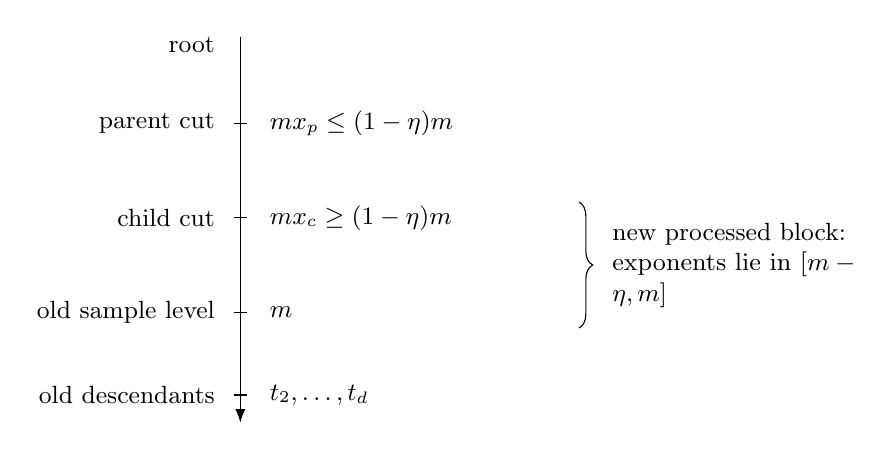
\begin{tikzpicture}[>=Latex,x=1cm,y=1cm,every node/.style={font=\small}]
 \draw[->] (0,0.45)--(0,-4.45);
 \node[anchor=east] at (-.2,.35) {root};
 \foreach \y/\label in {-.65/{parent cut},-1.85/{child cut},-3.05/{old sample level},-4.1/{old descendants}} {
  \draw (-.08,\y)--(.08,\y);
  \node[anchor=east] at (-.2,\y) {\label};
 }
 \node[anchor=west] at (.25,-.65) {$m x_p\le(1-\eta)m$};
 \node[anchor=west] at (.25,-1.85) {$m x_c\ge(1-\eta)m$};
 \node[anchor=west] at (.25,-3.05) {$m$};
 \node[anchor=west] at (.25,-4.1) {$t_2,\ldots,t_d$};
 \draw[decorate,decoration={brace,amplitude=5pt}] (4.3,-1.65)--(4.3,-3.25);
 \node[anchor=west,align=left,text width=3.1cm] at (4.6,-2.45)
  {new processed block:\\exponents lie in $[m-\eta,m]$};
\end{tikzpicture}
\caption{One structural transition when both cuts are proper. The parent
exponent decreases by a fixed factor; the levels strictly below it through
the old sample level form the new processed block. The cut parameters are
$x_p=\Prob(Q<q)$ and $x_c=\Prob(Q<r)$. Trivial parent or child cuts are
omitted, as specified in the proof. The old descendant row is absent when
$d=1$.}
\label{fig:hidden-cuts}
\end{figure}


Panchenko's pure-state theorem proves hierarchical exchangeability of spin
arrays and their independence from cluster weights under spin-tested
Ghirlanda--Guerra identities~\cite[Theorem~1]{Panchenko2015HE}.
To describe the corresponding indexing here, rank cut clusters by decreasing
frequency within their parents, resolving ties by the least natural sample
index, and list samples within each deepest cluster in natural order.
Write $(\alpha,l)\in\N^h\times\N$ for a sample's new address: $\alpha$
is its hidden-cluster address and $l$ its number within that cluster.
The decoration array becomes $D'_{\alpha,l,\xi,i}$. The whole old
descendant subtree moves with its first-level sample $u$; the site index
$i$ stays common. The following local argument proves independence of
this reindexed array from the full partition that determines its addresses.

\FloatBarrier
\begin{lemma}[The marked cut representation]\label{ct:marked-cuts}
The nested cut partition has the sample-partition law of an RPC with
parameters \eqref{ct:cut-parameters}. The reindexed decorations
$D'_{\alpha,l,\xi,i}$ are independent of the full partition and are
hierarchically exchangeable in the hidden-cluster and sample coordinates.
They retain the independent hierarchical exchangeabilities of the old
descendant trees and the simultaneous exchangeability of the sites.
\end{lemma}

\begin{proof}
For a cut of parameter $x_j$, let $C$ be a cluster seen among the
first $n$ samples, of size $n_C$.  Select an anchor in $C$ by a
finite case distinction.  Equation~\eqref{ct:marked-gg}, with
the indicator of the anchor's cut relation as $\psi$, shows that,
conditionally on all past pair and decoration data, the next
sample belongs to $C$ with probability
\begin{equation}\label{ct:partition-prediction}
                            \frac{n_C-x_j}{n}.
\end{equation}
Indeed the independent term contributes $(1-x_j)/n$ and the past
anchor-neighbor terms contribute $(n_C-1)/n$.  Differences between
these probabilities specify the creation of new children within
each parent.  These are exactly the RPC predictions in
Lemma~\ref{ctr:rpc}, Equation~\eqref{ctr:prediction}.  They determine every
finite nested
partition law.  Consequently the full partition has that law, its
clusters have positive frequencies, and the frequencies at every
level have total mass one.  The ranked leaf frequencies have the
corresponding RPC distribution.  For $h=0$ these statements mean a
single cluster of mass one.

We now prove independence from the full partition using the decoration
tests in Equation~\eqref{ct:marked-gg}.  Let $I$ be a deterministic
ordered tuple of distinct sample indices, let $D_I$ be all their
decorations, and let $\Pi$ be the full nested partition.  Expose $I$
first, using exchangeability.  Given its cut pattern and decorations,
iterating \eqref{ct:partition-prediction} shows that the conditional
law of the partition on all remaining indices depends only on that
cut pattern.  In this iteration one can condition down from all
intermediate decorations, since the predictions do not depend on them.
Extending from finite restrictions to the countable partition gives,
for every bounded decoration test $f$,
\begin{equation}\label{ct:conditional-decoration-law}
 \E[f(D_I)\mid\Pi]=K_{\Pi|_I}(f),
\end{equation}
where the probability kernel $K$ depends only on the ordered internal
cut pattern $\Pi|_I$, and not on the actual values of the indices.

The inverse image of a fixed finite tuple of distinct positions in
the ranked-cluster/natural-order indexing is a tuple of original
indices measurable with respect to the partition.  Partitioning
according to its countably many possible values and applying
Equation~\eqref{ct:conditional-decoration-law} proves that the reindexed tuple's decoration
law is independent of the partition.  Its internal cut pattern is
fixed by its new positions.  The same argument shows invariance
under ancestry-preserving permutations of the hidden clusters and
of the sample indices within them.  It applies to arbitrary finite
decoration cylinders and hence to the complete arrays.  The old
descendant permutations and the site permutations do not change
the cut partition, so their invariances are retained as well.
\end{proof}

We have now separated the RPC partition from the complete decoration
array.  The next representation supplies path variables for that array.

Combine the $h$ hidden levels, the sample level, and the $d-1$ old
descendant levels into one label tree of depth $h+d$.  Together with
the depth-one site tree, the decorations form an array on a product
of two finite-depth, countably branching trees.  Their entry space,
a finite product of compact type spaces, is standard Borel.
The invariances just proved give the separate ancestry-preserving
permutation invariances for these two trees.
Theorem~2 of Austin and Panchenko~\cite{AustinPanchenko2014} therefore
represents this array by measurable functions of independent uniform
variables indexed along the product of the two ancestor paths.
Those paired with the site-tree root are shared globals $z_l$;
those paired with site $i$ are site variables $u_{l,i}$.
We take this representation independent of the partition, as
permitted by Lemma~\ref{ct:marked-cuts}.  All shared globals are
retained, including the root global.  The representation concerns the
site array alone; fresh packet counts and signs are still drawn
independently at the root, as in Section~\ref{ctr:section}.

An old type at a boundary shifted by $h$ has a version using only
the variables through that boundary.  To see this, take two leaves
agreeing through the boundary and diverging immediately afterward.
Their boundary-type entries, for the same site, are equal almost
surely by the duplicated-entry property.  In the representation
these two entries are conditionally independent and identically
distributed given the prefix variables.  Their conditional law is
therefore a point mass.  A measurable version depends only on the
prefix.  There are only countably many entries, so these versions
agree simultaneously throughout the array.  At the last boundary
there is no reduction to make.

\subsection{Identifying the endpoint functional}\label{ct:sub-endpoint}

The representation just obtained has new levels.  We determine their
exponents and their endpoint values from the original natural-order
sampling.  This calculation uses the full array law behind the finite
partition, including the distribution within its bands.

\begin{lemma}[Uniform empirical tree evaluation]\label{ct:empirical}
Let $C\ge0$, let $B\ge1$ be an integer, and let $|X|\le C$ in a hierarchy of fixed depth $d$ with
exponents in $(0,1]$.  At every vertex replace its conditional integral
by the empirical average over $B$ conditionally independent children.
The resulting nested logarithmic transform differs from the exact
transform in mean absolute value by at most
\[
                            A(C,d)B^{-1/2},
\]
uniformly in the conditional sampling kernels, the exponents, and
the root data.  The same statement holds for finitely many sites
sampled jointly at every vertex.
\end{lemma}

\begin{proof}
For a one-step transform of a random variable $Y\in[-C,C]$,
\[
 T_tY=\frac1t\log\E e^{tY},
 \qquad
 \widehat T_tY=\frac1t\log\left(\frac1B\sum_{b=1}^B e^{tY_b}\right).
\]
The standard deviation of $e^{tY}$ is at most $2tCe^C$, while
$t^{-1}\log v$ is $e^C/t$-Lipschitz on
$[e^{-tC},e^{tC}]$.  Hence
\begin{equation}\label{ct:one-step-empirical}
                      \E|\widehat T_tY-T_tY|
                              \le2Ce^{2C}/\sqrt B.
\end{equation}
If exact child values $Y$ are replaced by values $Y'$ in $[-C,C]$,
interpolation between the two sets of values gives
\[
               |T_tY-T_tY'|\le e^{2C}\E|Y-Y'|,
\]
and the identical bound with an empirical mean holds for an
empirical transform.  Apply these bounds recursively from the
leaves upward.  Every intermediate value remains in $[-C,C]$,
so the constants depend only on $C,d$.  A joint child variable
may include the global coordinate and all the finitely many site
coordinates; conditional independence between children is all that
was used.
\end{proof}

\begin{lemma}[Endpoint passage]\label{ct:endpoint}
Equip the represented hierarchy with exponents
\begin{equation}\label{ct:new-exponents}
                  mx_1,\ldots,mx_h,\ m,\ t_2,\ldots,t_d.
\end{equation}
For each endpoint of horizon $k$, its expected nested transform is
the subsequential limit of the corresponding selected posterior
endpoint.  In particular its trial functional satisfies $G_k/k\le U$.
The hidden list is omitted when $h=0$, and the old descendant list is
omitted when $d=1$.
\end{lemma}

\begin{proof}
First fix all packet counts and signs, so the endpoint uses finitely
many distinct sites and its loss $X$ is bounded, say by $C$.
For each fixed $B$, the empirical tree evaluation is a continuous
function of finitely many retained message values and of the old
exponents.  Continuity follows also at messages equal to zero or
one, because every factor $1-wf_1f_2f_3$ is at least
$1-w=e^{-\beta}>0$.  The old exponents converge to positive limits
since $t_j\ge m_0$.
Thus weak convergence of the natural-order arrays gives convergence
of the expected empirical evaluation.  Lemma~\ref{ct:empirical}
is uniform before the limit, so taking $B\to\infty$ afterward
recovers exactly the subsequential expected endpoint value.

We now evaluate that same limit using the representation and its
independent cut partition.  Below the sample level, replace
empirical evaluations by the true conditional transforms
$T_{t_2},\ldots,T_{t_d}$.  The error tends to zero by the same
uniform estimate, even after propagation through the top empirical
average.  Write $Y_{\alpha,l}\in[-C,C]$ for the resulting value at
sample position $(\alpha,l)\in\mathbb N^h\times\mathbb N$.
Condition on the full cut partition and on all represented variables
through the hidden levels, including their root variables.  The
remaining sample-level variables are independent across sample
positions, and their laws are identical within each hidden leaf.
If $\alpha(u)$ is the leaf containing natural sample $u$, then
the conditional mean of the first-$B$ natural-order average is
\[
  \frac1B\sum_{u=1}^B
          \E_{\rm sample}e^{mY_{\alpha(u),1}}.
\]
Its conditional variance is $O_C(B^{-1})$.  The empirical
frequencies of the hidden leaves converge to their masses
$(v_\alpha)$; convergence is in $\ell^1$, since these are
probability masses whose pointwise limits have sum one.  Hence,
in $L^1$,
\begin{equation}\label{ct:natural-average}
 \frac1B\sum_{u=1}^B e^{mY_{\alpha(u),l(u)}}
   \longrightarrow
       \sum_\alpha v_\alpha\E_{\rm sample}e^{mY_{\alpha,1}}.
\end{equation}
Boundedness makes passage to the divided logarithm legitimate.
For $h=0$ the sum consists of one term of weight one.

Set $V_\alpha=T_m^{\rm sample}Y_{\alpha,1}$.  The represented marks
and their root variables were chosen independently of the full partition,
so the RPC weights retain their original law conditional on those root
variables and are independent of the attached marks.  If $h=0$, the
divided logarithm in \eqref{ct:natural-average} is simply
$V_{\varnothing}$, where $\varnothing$ is the unique empty label.
If $h\ge1$, the hidden parameters satisfy
$0<x_1<\cdots<x_h<1$, exactly the strict cascade hypothesis of
Lemma~\ref{ctr:rpc}.  Applying its logarithmic identity conditionally on
the root data to marks $mV_\alpha$ shows that
the expectation of the divided logarithm on the right of
\eqref{ct:natural-average} is the nested transform with hidden
exponents $mx_1,\ldots,mx_h$, followed by the sample exponent $m$.
The scaling is the identity
\[
                            T_x(mV)=mT_{mx}V,
\]
applied successively at the hidden levels and followed by division
by $m$.  Below them remain the old exponents $t_2,\ldots,t_d$.
This proves precisely \eqref{ct:new-exponents}.  The hidden exponents,
when present, are increasing and lie strictly between zero and $m$.
Every old descendant exponent is at least $m$, and their old order
persists.  Thus these are admissible intermediate trial exponents,
including when some old exponents coincide or equal one.

Finally remove the conditioning on counts and signs.  Both the
prelimit and limit transforms are bounded in absolute value by
$k\log2+\beta\sum D_i$, with the fixed Poisson packet laws.
Their tails are uniformly integrable.  Truncating counts, applying
the proved finite-count assertion, and then removing the truncation
establishes the assertion for each expected endpoint.  Subtracting
the B endpoint from the A endpoint and using
\eqref{ct:selected-value} yields $G_k/k\le U$.
\end{proof}

\subsection{Passing the pathwise structural records}\label{ct:sub-records}

The endpoint calculation has supplied a trial with the required value
bound.  It remains to preserve the old records and to construct the new
one.  We will pass empirical products of site tests through the weak
limit; the following Hilbert-space fact then converts those pairwise
bounds into statements about almost every individual global path.

\begin{lemma}[Closed support bounds]\label{ct:support}
Let $V,V'$ be independent random variables with the same law in a
separable Hilbert space, and let $\delta,\varepsilon\ge0$.
\begin{enumerate}
\item If $|\langle V,V'\rangle|\le\delta^2$ almost surely, then
      $\|V\|\le\delta$ almost surely.
\item If $\langle V,V'\rangle$ almost surely belongs to a fixed closed
      interval of length $\varepsilon$, then the support of their
      common law has diameter at most $\sqrt{2\varepsilon}$.  Consequently
      $\|V-\E V\|\le\sqrt{2\varepsilon}$ almost surely whenever
      the expectation exists.
\end{enumerate}
If $V,V'$ are conditionally independent with the same conditional law
given a standard Borel random element, the corresponding conclusions
hold for almost every conditional law in which the stated pair bound holds.
\end{lemma}

\begin{proof}
A closed set of full product measure contains the product of the
two supports: otherwise a pair of support points has product
neighborhoods of positive measure disjoint from that set.
The first assertion follows by putting the same support point in
both coordinates.  In the second, for support points $v,v'$, both
squared norms and their inner product belong to the same interval,
so
\[
 \|v-v'\|^2=\|v\|^2+\|v'\|^2-2\langle v,v'\rangle
                              \le2\varepsilon.
\]
Jensen's inequality gives the assertion about the barycenter.
The same reasoning applies after disintegration; separability
ensures that the relevant supports have full measure.
\end{proof}

\begin{lemma}[Preservation of the old records]\label{ct:old-records}
Every old processed block satisfies Equation~\eqref{ctr:record}
in the represented hierarchy, with the same test family and
tolerance and with its boundaries shifted by $h$.
\end{lemma}

\begin{proof}
Let $(b,c]$ be an old block.  Since the input hierarchy is active,
$b\ge1$.  In the prelimit natural array we may therefore choose
two paths in the same first-level sample, agreeing through $b$
and diverging immediately afterward.  At site $i$, form the
product of their two values of
\[
                              \phi(S_c)-S_b(\phi),
                         \qquad \phi\in\Phi_j.
\]
Condition on the complete globals of the two paths.  The sites
are independent and identically distributed, and the conditional
mean of this product is the $L^2(\dd u_{0:b})$ inner product of
the two error functions
\[
    E_z(u_{0:b})=
          \int\phi(S_c)\,\dd u_{b+1:c}-S_b(\phi).
\]
The fresh site variables after the branching point are independent
on the two paths; their shared site variables are exactly those
through $b$.  Equation~\eqref{ctr:record}, which survived the
posterior and Gaussian changes of law, bounds both error norms
by $\delta$.  Cauchy--Schwarz therefore bounds the absolute
conditional mean by $\delta^2$.

Let $M_I$ be the empirical mean over the first $I$ sites.  The
summands belong to $[-1,1]$, so
\begin{equation}\label{ct:old-empirical-bound}
     \E\operatorname{dist}(M_I,[-\delta^2,\delta^2])^2\le I^{-1}.
\end{equation}
For fixed $I$, the integrand on its left is a bounded continuous function of finitely
many retained type values: $\phi$ is continuous, and evaluation
of a probability measure against $\phi$ is continuous in the
type-space topology.  The inequality thus passes to the limit.
On $I=2^j$, Markov's inequality and Borel--Cantelli imply that
the displayed distance tends to zero almost surely.  This holds
simultaneously for all countably many path choices and all the
finitely many tests.  It consequently remains true for the
partition-selected paths after reindexing.

In the product-tree representation, the conditional strong law
for the sites identifies the limit of $M_I$ with the inner
product of the analogous error vectors, now in
$L^2(\dd u_{0:b+h})$.  Conditional on the common globals through
the shifted block start, those two vectors are independent and
identically distributed as their continuation globals vary.
Thus their inner product has absolute value at most $\delta^2$
almost surely.  Apply the first assertion of
Lemma~\ref{ct:support} to this conditional law.  Each error
vector has norm at most $\delta$ for almost every global
continuation.  Fubini's theorem gives precisely
Equation~\eqref{ctr:record} for almost every complete global
path.  The weak-limit step used a closed finite-column condition;
the pathwise conclusion then followed from the conditional support bound.
\end{proof}

Thus every previously processed block retains its record.  For the new
block, the narrow support band will provide the corresponding pairwise
bound without a preexisting record.

\begin{lemma}[A new processed block]\label{ct:new-record}
Let $c=h+1$ be the sample level.  Let $b=1$ if the parent cut is
present, and let $b=0$ otherwise.  There is an ancestor-measurable
probability-valued type $S_b$ such that $(b,c]$ satisfies
Equation~\eqref{ctr:record} for the specified new test family
and tolerance $\delta$.  Its exponents lie in $[m-\eta,m]$.
If the parent cut is present, its exponent belongs to
$(0,(1-\eta)m]$.
\end{lemma}

\begin{proof}
For two distinct natural first-level samples, average over the
first $I$ sites the product of their $\phi_j(S_1)$ values.
Conditional on their globals and Gaussian fields, the site's
root variable is shared between the two samples, and its
first-level variables are independent.  The conditional mean
is exactly $Q_j$ from \eqref{ct:features}.  Therefore
\begin{equation}\label{ct:new-empirical-bound}
       \E\left|\frac1I\sum_{i=1}^I
              \phi_j(S_1^{1,i})\phi_j(S_1^{2,i})-Q_j(1,2)
          \right|^2\le I^{-1}.
\end{equation}
For each fixed $I$ this inequality passes by continuity to the
natural-order limit array.  Along dyadic $I$, it gives almost-sure
convergence of the empirical average to $Q_j$, simultaneously
for all pairs and tests.

After reindexing, take two sample positions agreeing through $b$
and diverging immediately below $b$.  If the parent is present,
they are in the same parent cluster; otherwise $\Prob(Q<q)=0$.
If the child is present, they lie in distinct child clusters;
otherwise $\Prob(Q<r)=1$.  Consequently their natural pair
overlap satisfies $q\le Q<r$ almost surely in all cases.
By \eqref{ct:quantile-band} and
Lemma~\ref{ct:ordering}, the corresponding $Q_j$ belongs to
a fixed closed interval $I_j$ of length at most $J_f\gamma$.
The empirical characterization just proved shows that this
interval condition is a property of the reindexed decorations
alone; we do not need a separate representation of the kernels
$Q_j$.

In the product-tree representation, the site empirical limit is
the inner product in $L^2(\dd u_{0:b})$ of the two vectors
\begin{equation}\label{ct:new-vectors}
          A_j(u_{0:b})=
                     \int\phi_j(S_c)\,\dd u_{b+1:c}.
\end{equation}
Conditional on the ancestor globals through $b$, these are
independent copies as their continuation globals vary.
Their inner product belongs to $I_j$ almost surely.
The second assertion of Lemma~\ref{ct:support} shows that
the conditional support of $A_j$ has diameter at most
$\sqrt{2J_f\gamma}$.

Define, for each ancestor global and site history,
\begin{equation}\label{ct:new-type}
 S_b(z_{0:b},u_{0:b})
       =\operatorname{Law}_{z_{b+1:c},u_{b+1:c}}(S_c).
\end{equation}
All continuation variables in this formula have their current
independent uniform laws.  This is a measurable probability
kernel on the type space of $S_c$, hence has exactly the required
next type space.  By Fubini's theorem,
$S_b(\phi_j)$ is the conditional continuation-global barycenter
of the vector $A_j$ in \eqref{ct:new-vectors}.  The support
diameter bound gives
\[
  \int\left|
           \int\phi_j(S_c)\,\dd u_{b+1:c}-S_b(\phi_j)
      \right|^2\dd u_{0:b}\le 2J_f\gamma
\]
for almost every complete global path.  Choose
$0<\gamma\le\delta^2/(2J_f)$ to obtain the new record.

It remains to check the exponent band.  The only possible
intermediate level between $b$ and $c$ is the child cut, whose
exponent is $mx_c$.  By \eqref{ct:quantile-band},
$x_c\ge1-\eta$, so $m-mx_c\le m\eta\le\eta$.
The end exponent is $m$.  If the parent is present, its exponent
satisfies $0<mx_p\le(1-\eta)m$, as claimed.

The type in \eqref{ct:new-type} is defined once, at this
transition.  In subsequent posterior changes it is retained as
the same measurable function; it is not redefined by averaging
under the changed global law.  The pathwise record just proved
then survives by absolute continuity, exactly as do the old
records.
\end{proof}

\begin{proof}[Completion of the proof of Lemma~\ref{ct:transition}]
The compactness and representation construction inserts at most
two levels.  Lemma~\ref{ct:endpoint} supplies the limiting expected
endpoint values and $G_k/k\le U$.
Lemma~\ref{ct:old-records} preserves every old record, while
their exponent-band inequalities survive ordinary limits.
Lemma~\ref{ct:new-record} supplies the new processed block.
If there is no parent cut it begins at the root and processing
is complete.  Otherwise the hierarchy is active, its first
exponent is $mx_p>0$, and this is at most $(1-\eta)m$.
All records hold for almost every complete global path.  These constructions were made for the fixed output
horizon $k$; repeating them for any other fixed horizon proves
the asserted quantifiers.  All nonroot shared globals remain in this
output.  The next section removes them by a separate approximation
argument.
\end{proof}

\section{Removing the shared variables and completing the trials}\label{cc:section}

The transition in Lemma~\ref{ct:transition} keeps the shared variables
and preserves the conditional records. We now use it finitely many times,
then replace the nonroot shared variables by independent site sampling.
The order matters: the replacement estimate is for one packet, so we first
reduce the trial to a one-packet horizon. The final step approximates the
resulting conditional sampling laws by finite rational tables.

Panchenko's theorem for finite replica symmetry breaking~\cite[arXiv version, Theorem~2]{Panchenko2015FRSB}
removes common nonroot coordinates while retaining common root data, under
spin-tested Ghirlanda--Guerra identities, cavity equations for a modified
Hamiltonian, and an overlap law with finitely many exact values.
Here the overlap cuts partition a possibly continuous distribution.
The recorded conditional laws and the quantitative estimates below provide
the approximation needed to construct finite rational trials.

Panchenko's spin-distribution formula optimizes over a wider invariant
distributional class in its stated even-arity setting; its shared-coordinate
obstruction is explicit after Lemma~6
\cite[arXiv version, Theorem~2 and the Remark after Lemma~6]{Panchenko2013SD}.

\subsection{From recorded tests to probability kernels}

Write $W_1$ for the Wasserstein metric associated with the metric on a
compact type space.  Every iterated type space $K^{(j)}$ in
the structural record~\eqref{ctr:record} is compact and has diameter
at most one. Write $z=(z_0,\ldots,z_d)$ for a complete global path.

\begin{lemma}[Finite tests for the site law]\label{cc:site-law}
Given $e_0>0$ and a finite nonempty list of type spaces, one can choose finite
nonempty collections $\Phi_j$ of $[0,1]$-valued $1$-Lipschitz functions
such that, for probability measures $\nu,S$ on $K^{(j)}$,
\begin{equation}\label{cc:net-bound}
 W_1(\nu,S)
 \le\max_{\phi\in\Phi_j}|\nu(\phi)-S(\phi)|+e_0/2.
\end{equation}
If the structural record holds with
\begin{equation}\label{cc:delta-choice}
 \bigl(\max_j|\Phi_j|\bigr)\delta\le e_0/2,
\end{equation}
then, for each processed block $(b,c]$ and almost every fixed global
path,
\begin{equation}\label{cc:site-law-distance}
 \int W_1\bigl(\nu_{z,u_{0:b}},S_b(z_{0:b},u_{0:b})\bigr)
               \,\dd u_{0:b}\le e_0.
\end{equation}
Here $\nu_{z,u_{0:b}}$ is the conditional law of $S_c$ obtained by
integrating only the fresh site coordinates $u_{b+1:c}$, with all the
global coordinates fixed.
\end{lemma}

\begin{proof}
Kantorovich--Rubinstein duality expresses $W_1$ as the supremum of
integral differences over $1$-Lipschitz functions.  Constants cancel from
such differences; since the space has diameter at most one, each test
can be shifted into $[0,1]$.  The class of these bounded Lipschitz
functions is compact in the uniform norm.  A finite $e_0/4$-net gives
Equation~\eqref{cc:net-bound}, since replacing a test by a net point
changes the difference of its two integrals by at most $e_0/2$.

For a fixed test, the structural record and Cauchy--Schwarz give
\[
 \int |\nu_{z,u_{0:b}}(\phi)-S_b(z_{0:b},u_{0:b})(\phi)|
                 \,\dd u_{0:b}\le\delta.
\]
Bound the maximum over tests by their sum, integrate
Equation~\eqref{cc:net-bound}, and use
Equation~\eqref{cc:delta-choice}.  This proves
Equation~\eqref{cc:site-law-distance} with its almost-everywhere global
quantifier intact.
\end{proof}

\subsection{Finite stopping}

\begin{proposition}[A terminal one-packet trial]\label{cc:terminal}
Fix $U>P(a,\beta)$, $0<\eta,m_0<1$, and an integer $J$ such that
\begin{equation}\label{cc:stopping-depth}
 (1-\eta)^J<m_0.
\end{equation}
Choose in advance finite nonempty test sets on $K^{(j)}$, $0\le j\le J$,
and a structural tolerance $\delta>0$.  For every $\rho>0$ there is a
trial with
\[
 G_1\le U+\rho,
\]
at most $J$ processed blocks, and depth at most $2J+1$, which satisfies
the chosen structural records and has one of the following forms:
\begin{enumerate}
 \item the processed blocks start at the root boundary $0$;
 \item the processed blocks start at boundary $1$, and the remaining
       first exponent satisfies $0<m<m_0$.
\end{enumerate}
Every processed block has exponent width at most $\eta$.
\end{proposition}

\begin{proof}
Lemma~\ref{ctr:reservoir} supplies trials for arbitrarily large
integer horizons $N$, initially of depth one and first exponent $1$,
with $G_N/N\le U$.  There are initially no processed blocks.  A trial
is terminal if its blocks start at the root or if its first unprocessed
exponent is less than $m_0$.

Suppose a sequence at a given stage contains no terminal trial.  All its
first exponents are then at least $m_0$.  Depth has increased by at most
two at each preceding transition, so there are only finitely many
possible patterns of block boundaries.  Pass to an unbounded horizon
subsequence with a common pattern, and then to a subsequence on which
the exponents converge.  Lemma~\ref{ct:transition}, with its
fixed tests and tolerance, produces for each fixed positive integer $k$
an output trial satisfying $G_k/k\le U$.  It preserves the old records
and adds one processed block.  Either the output is terminal, or its
new first exponent is at most $(1-\eta)$ times the limiting old first
exponent.

This use of the transition involves nested limits, not a uniform limit
in $k$.  First fix $k$; then take the input horizon to infinity as
required by the transition; finally retain an output for that $k$.
Doing this separately for $k=1,2,\ldots$ gives the next unbounded
horizon sequence if no terminal output occurs.  After $j$ transitions
every still-active output has first exponent at most $(1-\eta)^j$.
Equation~\eqref{cc:stopping-depth} therefore forces termination after
at most $J$ transitions.  The resulting terminal trial has some finite
horizon, at most $J$ blocks, and depth at most $2J+1$.

Reduce its horizon to one using the packet telescope of
Lemma~\ref{ctr:posterior}, without a Gaussian perturbation.  There is
no remainder when the blocks have size one.  The sum of the averaged
one-packet posterior differences is the original $G_k$, so one step,
and then base root data outside the conditional null sets, have
posterior value at most $U+\rho$.  This selection is made before fresh
packet data are sampled.  The conditional laws generated by the
posterior densities remain equivalent to the old laws, and the old
site-law functions are kept rather than recomputed.  Hence all the
almost-everywhere records persist.  Neither the exponents nor the
terminal boundary changes.  This gives the asserted one-packet trial.
\end{proof}

\subsection{Removing shared variables after stopping}

\begin{lemma}[Collapse by the recorded kernels]\label{cc:kernel-collapse}
Consider a terminal trial from Proposition~\ref{cc:terminal}, whose
records imply Equation~\eqref{cc:site-law-distance}.  Fix a count cutoff
$D_0\ge1$ and put
\[
 C=\log2+\beta D_0,\qquad M=3D_0,
 \qquad
 R=JM e^\beta e^{2C(2J+2)}e_0.
\]
There is a site-only trial, with weakly increasing exponents in $(0,1]$,
such that
\begin{equation}\label{cc:collapse-error}
 |G_1^{\mathrm{site}}-G_1|
 \le 2K(C)\eta+2R+C^2e^{2C}m_0+2\tau_A+2\tau_B,
\end{equation}
where
\[
 \tau_A=\E[(\log2+\beta D_A)\1_{\{D_A>D_0\}}],\qquad
 \tau_B=\E[(\log2+\beta D_B)\1_{\{D_B>D_0\}}],
\]
with $D_A\sim\Poi(3a)$ and $D_B\sim\Poi(2a)$.
In the root-terminal case the term containing $m_0$ is unnecessary.
The new message kernels are independent of the fresh packet counts
and signs.
\end{lemma}

\begin{proof}
We first condition on either endpoint's fresh count and sign data with
$D\le D_0$.  Its loss $X$ is bounded in absolute value by $C$, and it
uses at most $M$ distinct reservoir occurrences.  Simultaneously replace
all exponents in each processed block $(b,c]$ by $t_c$.  The resulting
vector is still nondecreasing and is within $\eta$ of the original.
Lemma~\ref{cs:sensitivity} bounds the change by $K(C)\eta$.
A block with constant exponent is one conditional $T_{t_c}$ operation
over all its coordinates, by the tower property.

Define deterministic functions of vectors of single-site types,
one coordinate for each reservoir occurrence, working upwards through
the block boundaries.  At the last boundary put
$F_d(\mathbf S_d)=X$.  For a block $(b,c]$ put
\begin{equation}\label{cc:kernel-recursion}
 F_b(\mathbf s)=\frac1{t_c}\log\int
       \exp\bigl(t_cF_c(\mathbf u)\bigr)\prod_i s_i(\dd u_i).
\end{equation}
These functions depend on the fixed count and sign data, but the
probability kernels $S_b$ do not.  The functions $F_b$ are bounded in
absolute value by $C$.

Use the sum metric on each finite product of type spaces.  The terminal
loss is $e^\beta$-Lipschitz: a clause factor is bounded below by
$1-w=e^{-\beta}$, the product of at most three $[0,1]$ messages changes
by at most the sum of their changes, and the log-sum-exp for the two
branches of an A packet preserves the largest branchwise log error.
Thus we may take $L_d=e^\beta$ as a Lipschitz constant for $F_d$.
Coordinatewise couplings in Equation~\eqref{cc:kernel-recursion} give
\begin{equation}\label{cc:lipschitz-recursion}
 L_b\le e^{2C}L_c.
\end{equation}
Indeed $v\mapsto e^{t_cv}$ has Lipschitz constant at most $t_ce^C$ on
$[-C,C]$, and the divided logarithm on the possible integral values
has Lipschitz constant at most $e^C/t_c$.  The same two bounds show that
a mean absolute error in an inside value propagates through a block
by at most the factor $e^{2C}$.

Let $Y_b$ denote the actual effective value at boundary $b$ after
flattening the processed blocks' exponents.  Thus $Y_d=X$, and across
a block $(b,c]$ the value $Y_b$ is the conditional $T_{t_c}$ average
of $Y_c$ over the block's global and site coordinates.  Define
\[
 E_b=\E_{\mathrm{base}}
       \bigl|Y_b-F_b(\mathbf S_b)\bigr|.
\]
Here the expectation uses the current trial law on the global history
and all occurrences' fresh site histories through $b$, before any
exponential reweighting by this fresh packet.  This law already includes
any old-packet posterior used to obtain the trial; the packet count and
signs remain fixed.  In particular $E_d=0$.  We claim that
\begin{equation}
 E_b\le e^{2C}E_c+e^{2C}L_cMe_0.
 \label{cc:one-block-error}
\end{equation}

First replace $Y_c$ inside the block average by
$F_c(\mathbf S_c)$.  The mean-error propagation bound above gives
the first term of Equation~\eqref{cc:one-block-error}.  To bound the remaining error, fix the
ancestor histories through $b$ and the continuation globals through
$c$.  Under this conditioning, the occurrences' fresh site
continuations are independent; write $\nu_i$ for the resulting law
of $S_c^i$.  A product of Wasserstein couplings and the Lipschitz
constant of $F_c$ give
\[
 \left|\int e^{t_cF_c(\mathbf u)}\prod_i\nu_i(\dd u_i)
       -\int e^{t_cF_c(\mathbf u)}\prod_iS_b^i(\dd u_i)\right|
 \le t_ce^C L_c\sum_i W_1(\nu_i,S_b^i).
\]
The second integral depends only on the ancestor histories.  Average
this inequality over the continuation globals, apply the
$e^C/t_c$ Lipschitz bound for the divided logarithm, and then average
over the ancestor histories.  For almost every fixed global path,
Equation~\eqref{cc:site-law-distance} bounds the integral over each
occurrence's site ancestors by $e_0$.  The continuation-global law
is independent of these fresh site generators, including when the
trial was obtained by a posterior change of law.  Fubini's theorem
therefore bounds the final average by $e^{2C}L_cMe_0$ and proves Equation~\eqref{cc:one-block-error}.

There are at most $J$ processed blocks, and
$L_c\le e^{2CJ}e^\beta$ at every boundary.  Iterating Equation~\eqref{cc:one-block-error} from
$E_d=0$ bounds their accumulated error.  If the starting boundary
is $1$, propagating once through the remaining first-level transform
adds at most one factor $e^{2C}$.  In either case the error is at most
\[
 JM e^\beta e^{2C(2J+2)}e_0=R.
\]

If the processed blocks begin at the root, the resulting recursion
already describes a site-only trial. Retain the common root $z_0$
and sample each occurrence's initial type $S_0(z_0,u_0^i)$ using its
own fresh root-site uniform. At one level of exponent $t_c$ for each
old block, draw each site's next type independently from its preceding
type, and continue to the message pair.  Probability kernels on these compact metric spaces
can be sampled by measurable functions of fresh uniform variables.
This construction evaluates Equation~\eqref{cc:kernel-recursion}.

If the blocks begin at boundary $1$, there is still the operation
$T_mF_1(\mathbf S_1)$, where $0<m<m_0$.  Conditional on the root data,
factor this operation as
\[
 T_m^{z_1}T_m^{\mathrm{sites}}F_1(\mathbf S_1).
\]
The inside quantity is in $[-C,C]$.  By
Equation~\eqref{cs:small-exponent}, replacing the outside
$T_m^{z_1}$ by ordinary expectation changes its value by at most
$\tfrac12 C^2e^{2C}m_0$.  Move $z_1$, with this ordinary sampling law,
into the root global data.  Retain the level-$1$ site transform and
the independent block draws just constructed.  This is again
site-only.  Its kernels were constructed from the recorded types
alone, not from any fresh count or sign data.

For counts greater than $D_0$, both the old and new endpoint transforms
are bounded in absolute value by $\log2+\beta D$, regardless of their
kernels or exponents.  Their contribution to the difference is thus
at most twice the corresponding tail expectation.  Summing the
bounded-count estimates for the two endpoints proves
Equation~\eqref{cc:collapse-error}.
\end{proof}

\subsection{Rational finite descriptions}

\begin{theorem}[Finite rational completeness]\label{cc:complete}
\label{cc:rational}
For every $a>0$ and finite $\beta>0$,
\begin{equation}\label{cc:finite-infimum}
 P(a,\beta)=\inf_{\mathcal Q}G_1,
\end{equation}
where $\mathcal Q$ consists of site-only trials of finite depth whose
exponents are strictly increasing rationals in $(0,1)$ and whose
message pair is a rational-valued step function on a finite rational
rectangular grid in its root and site uniform variables.  In
particular, this is a countable class with an effective enumeration.
\end{theorem}

\begin{proof}
The upper bound of Proposition~\ref{ctr:upper} gives
$P(a,\beta)\le G_1$ for every member of $\mathcal Q$.  We prove the
reverse inequality by giving the order of all approximation choices.

Fix $\epsilon>0$ and put $U=P(a,\beta)+\epsilon$.  First choose a
count cutoff $D_0\ge1$ with $\tau_A,\tau_B\le\epsilon$, and set
$C=\log2+\beta D_0$.  Choose $\eta,m_0\in(0,1)$ so that
\[
 K(C)\eta\le\epsilon,\qquad
 \tfrac12 C^2e^{2C}m_0\le\epsilon.
\]
Next choose $J$ satisfying Equation~\eqref{cc:stopping-depth}, and
only then choose $e_0>0$ so small that
\[
 J(3D_0)e^\beta e^{2C(2J+2)}e_0\le\epsilon.
\]
Choose the finite test sets on all type spaces through $K^{(J)}$ by
Lemma~\ref{cc:site-law}, and finally choose $\delta$ satisfying
Equation~\eqref{cc:delta-choice}.  In particular, neither the test
precision nor the allowed number of transitions is chosen in response
to the eventual hierarchy depth.  The overlap widths used inside each
transition are chosen only after these test sets and $\delta$, as in
Lemma~\ref{ct:transition}.

Proposition~\ref{cc:terminal}, with $\rho=\epsilon$, gives a
terminal one-packet trial of value at most $P+2\epsilon$.
Lemma~\ref{cc:kernel-collapse} turns it into a site-only trial whose
value is at most $P+12\epsilon$: the exponent changes contribute at
most $2\epsilon$, the kernel replacements at most $2\epsilon$, the
possible small-exponent replacement at most $2\epsilon$, and the
two tails at most $4\epsilon$.

It remains to obtain a finite rational description.  Approximate the
finite weakly increasing exponent vector by strictly increasing
rational vectors in $(0,1)$.  This is possible even if some original
exponents coincide or equal $1$.  For fixed count data,
Lemma~\ref{cs:sensitivity} gives convergence of the
transform values.  The packet bound of
Equation~\eqref{ctr:packet-bound}, uniform over the approximations,
then gives convergence after averaging the Poisson counts and signs.

Encode the root randomness by a single uniform coordinate.  After the
independent conditional type samplings have likewise been encoded by
uniform coordinates, the message pair is a measurable function of
finitely many independent uniforms: the root global, the root site
coordinate, and the finitely many site-level coordinates.  Approximate
this pair in $L^1$ by rational-valued step functions on finite dyadic
rectangular grids.  For example, conditional expectations on the
successive dyadic grids converge in $L^1$, and subsequent rational
quantization preserves the range $[0,1]^2$ and the convergence.
The shared root coordinate is retained as shared; no independence
across sites is introduced there.

For fixed counts and signs, the leaf Lipschitz estimate in the proof
of Lemma~\ref{cc:kernel-collapse} bounds the mean leaf error by
$e^\beta$ times the sum of the $L^1$ message errors over the finitely
many occurrences.  The mean-error propagation bound through the
fixed finite hierarchy proves convergence of both endpoint values.
Once more, the root linear-in-count bound makes the Poisson tails
uniform, so their fully averaged $G_1$ values converge.  Thus a member
of $\mathcal Q$ has value at most $P+13\epsilon$.

Since $\epsilon$ is arbitrary, Equation~\eqref{cc:finite-infimum}
follows.  Finite depths, finite grids, rational exponents, and finite
rational tables all have finite encodings and can be enumerated by a
single ordinary algorithm.  These are the trials used in the
certificate search; none of the compactness limits or tolerance
choices in the existence proof is input to that search.  The larger class of strict measurable site-only trials contains
$\mathcal Q$ and obeys the same upper bound, so its infimum also equals
$P(a,\beta)$.
\end{proof}

\section{Completing the computation}\label{sec:assembly}

We now have the two certificate families described in
Section~\ref{sec:certificates}. Let $\alpha$ be the threshold constructed
in Theorem~\ref{cp:threshold}. Proposition~\ref{cp:finite-computation}
gives a computable rational sequence $(\ell_n)$ with
$\ell_n<\alpha$ and $\ell_n\to\alpha$. Its underlying finite-size bound
is the exact one-sided estimate
\[
 \frac{f_n}{n}-2^{67}n^{-1/6}\le\alpha.
\]
For the upper certificates, a rational trial is the finite site-only
description of Section~\ref{ctr:section}: it has strictly increasing
rational exponents in $(0,1)$ and a rational-valued message pair on a
finite rational rectangular grid of the root and site uniform variables.

\begin{lemma}[Upper certificates]\label{assembly:upper}
For positive rational $a$, positive integer $\beta$, and a rational trial
$Q$, the inequality $G_1(a,\beta;Q)<0$ certifies $\alpha\le a$.
Every rational $a>\alpha$ has such a certificate. The class of certified
densities is effectively enumerable.
\end{lemma}

\begin{proof}
The trial bound of Proposition~\ref{ctr:upper} gives
$P(a,\beta)\le G_1(a,\beta;Q)$. If $a<\alpha$, the pressure exists by
Lemma~\ref{ctr:pressure} and is nonnegative by Corollary~\ref{cp:soft-signs}.
Thus a negative trial is impossible below $\alpha$ and certifies the
non-strict inequality $\alpha\le a$. Nothing about the pressure at
equality is needed.

If $a>\alpha$, Corollary~\ref{cp:soft-signs} supplies a positive integer
$\beta$ for which $P(a,\beta)<0$. Theorem~\ref{cc:complete} says that
$P(a,\beta)$ is the infimum of the rational trial values. A rational
trial therefore has negative value. Its finite description is eventually
enumerated, and Lemma~\ref{ctr:evaluation} eventually gives a rational
interval for its value with negative upper endpoint. Enumerating positive
rational densities, positive integer penalties, finite descriptions and
accuracy indices gives the asserted enumeration.
\end{proof}

\begin{proof}[Proof of Theorem~\ref{thm:main}]
Theorem~\ref{cp:threshold} proves the strict-side probability limits for
the proper three-clause model in the introduction, with
$\alpha\in[1/200,10]$. Set $\alpha_3=\alpha$. This also identifies the
constant with the same-model $k=3$ threshold in
\cite[Theorem~1.1]{FixedClauseThreshold} by the uniqueness argument in
Section~\ref{sec:proof-map}.

Use the sequence from Proposition~\ref{cp:finite-computation} as the lower
sequence in Lemma~\ref{cert:search}, and use $G=G_1$ on the rational trial
class. This class is effectively enumerable by its finite encoding, and
Lemma~\ref{ctr:evaluation} proves uniform computability of its values.
Lemma~\ref{assembly:upper} proves both sign hypotheses of the search
lemma. Since $\alpha\in[0,20]$, all its assumptions hold. The resulting
single finite machine halts on every unary input $1^r$ and returns the
required binary-encoded rational within $2^{-r}$.

The compactness subsequences, conditional laws, Gaussian parameters and
approximation tolerances used to prove completeness are not inputs to the
machine. They establish the existence of finite witnesses, which the
search finds through its fixed enumeration. The running time of this fixed
machine on $1^r$ is itself a total computable function of $r$, obtained by
simulating the halting computation; the proof supplies no efficiency
estimate for that function.
\end{proof}

\bibliographystyle{plain}
\bibliography{references}
\end{document}
